\documentclass[14pt,a4paper]{extarticle}
\usepackage{amsmath,graphicx,booktabs,caption,placeins,setspace,titlesec}
\usepackage[left=30mm,right=15mm,top=20mm,bottom=20mm]{geometry}
\usepackage{fontspec}
\usepackage{polyglossia}
\setdefaultlanguage{russian}
\setmainfont{Liberation Serif}
\setmonofont{DejaVu Sans Mono}[Scale=MatchLowercase]
\usepackage[unicode,hidelinks]{hyperref}

\hypersetup{
  pdftitle={Волоконно-оптическая линия связи},
  pdfauthor={Ф. С. Кузькин, Н. М. Куприн}
}
\graphicspath{{figures/}}
\numberwithin{equation}{section}
\numberwithin{figure}{section}
\numberwithin{table}{section}
\captionsetup{font=small,labelsep=endash}
\captionsetup[figure]{name=Рисунок}
\captionsetup[table]{name=Таблица,justification=raggedright,singlelinecheck=false}
\titleformat{\section}{\centering\normalfont\bfseries}{\thesection}{1em}{}
\titleformat{\subsection}{\normalfont\large\bfseries\filright}{\thesubsection}{0.8em}{}
\setcounter{tocdepth}{3}
\onehalfspacing
\raggedright
\setlength{\parindent}{1em}

\newcounter{subsubsubsec}[subsubsection]
\renewcommand{\thesubsubsubsec}{\thesubsubsection.\arabic{subsubsubsec}}
\newcommand{\subsubsubsection}[1]{%
  \par\medskip\refstepcounter{subsubsubsec}%
  \noindent\textbf{\thesubsubsubsec\quad #1}\par\nobreak\smallskip
}
\newcommand{\dd}{\mathop{}\!\mathrm{d}}
% Численные результаты из analysis.py
\newcommand{\OverviewStep}{10}
\newcommand{\FineStep}{0{,}2}
\newcommand{\PeakEarly}{0{,}00}
\newcommand{\PeakLate}{3{,}40}
\newcommand{\PeakDelay}{3{,}40}
\newcommand{\DelayLower}{3{,}38}
\newcommand{\DelayUpper}{3{,}42}
\newcommand{\GroupIndex}{1{,}50}
\newcommand{\LengthMeters}{680}
\newcommand{\LengthKm}{0{,}680}
\newcommand{\LengthLower}{676}
\newcommand{\LengthUpper}{684}
\newcommand{\ReferenceIndex}{1{,}4682}
\newcommand{\ReferenceLength}{694}
\newcommand{\BackgroundLimit}{-0{,}60}
\newcommand{\WindowStart}{-1{,}5}
\newcommand{\WindowEnd}{8{,}0}
\newcommand{\AreaRatio}{0{,}853}
\newcommand{\PathLoss}{0{,}69}
\newcommand{\EffectiveLoss}{1{,}02}
\newcommand{\PulseRows}{%
  Короткое & 19 & \(-1{,}10502\) & 0,660 & 4,837 \\
  Длинное & 5 & \(-1{,}10618\) & 0,715 & 4,126 \\
}
\newcommand{\SensitivityRows}{%
  5,0 & Среднее & \(-0{,}60\) & 0,683 \\
  6,0 & Среднее & \(-0{,}60\) & 0,688 \\
  8,0 & Среднее & \(-0{,}60\) & 0,691 \\
  8,0 & Медиана & \(-0{,}60\) & 0,701 \\
  8,0 & Среднее & \(-1{,}00\) & 0,692 \\
}


\begin{document}
\begin{titlepage}
  \thispagestyle{empty}
  \begin{center}
    \textbf{Министерство науки и высшего образования Российской Федерации}

    \vspace{0.5cm}
    \textbf{НАЦИОНАЛЬНЫЙ ИССЛЕДОВАТЕЛЬСКИЙ ЯДЕРНЫЙ УНИВЕРСИТЕТ «МИФИ»}

    \vspace{0.5cm}
    Учебно-научный центр «Квантовый инжиниринг»

    \vspace{2cm}
    \textbf{ОТЧЁТ}

    по лабораторному практикуму «Квантовые технологии»

    \vspace{0.5cm}
    \textbf{Волоконно-оптическая линия связи}
  \end{center}

  \vspace{2.5cm}
  \begin{flushleft}
    \textbf{Студенты группы Б24-222}

    \textit{Ф.\,С. Кузькин, Н.\,М. Куприн}

    \vspace{0.8cm}
    \textbf{Преподаватель}

    \textit{Инженер К.\,С. Лукьянов}
  \end{flushleft}

  \vfill
  \begin{center}
    Москва 2026
  \end{center}
\end{titlepage}

\setcounter{page}{2}
{\small\tableofcontents}
\clearpage

\section*{ВВЕДЕНИЕ}
\phantomsection
\addcontentsline{toc}{section}{ВВЕДЕНИЕ}

Цель работы состоит в определении длины волоконной линии задержки
по разности времён прихода двух копий оптического импульса и в
оценке ослабления сигнала при прохождении через плечо с катушкой.

Волоконно-оптические линии обладают высокой пропускной способностью,
низким уровнем потерь и устойчивостью к электромагнитным воздействиям.
Затухание определяет запас мощности, необходимый для передачи
сигнала. В импульсном режиме измерение времени прохождения по
волокну позволяет определить протяжённость оптического пути.

\section{ТЕОРЕТИЧЕСКАЯ ЧАСТЬ}

\subsection{Структура и характеристики волоконно-оптических систем связи}

Передача информационных сигналов в волоконно-оптических линиях связи (ВОЛС) осуществляется посредством оптических кабелей (ОК). Базовым элементом ОК выступает волоконный световод (оптическое волокно)~- цилиндрический волновод из оптически прозрачного диэлектрика, обеспечивающий направленное распространение электромагнитных волн оптического диапазона.

Ключевые эксплуатационные преимущества ВОЛС, согласно \cite{Slepov,Burdin}, включают:
\begin{enumerate}
    \item широкую полосу пропускания, позволяющую передавать сигналы со скоростью до десятков Тбит/с и выше;
    \item низкий уровень потерь, обеспечивающий передачу без регенерации на расстояние порядка 200-300~км;
    \item высокую помехозащищённость и нечувствительность к электромагнитным помехам;
    \item малые массу и размеры кабелей;
    \item пожаробезопасность и отсутствие потребности в дефицитных проводниковых материалах;
    \item повышенную сложность несанкционированного перехвата передаваемых сообщений.
\end{enumerate}

Развитие ВОЛС стало возможным благодаря снижению потерь в оптических волокнах до значений, близких к теоретическому пределу, а также созданию полупроводниковых инжекционных лазеров (ИЛ) с непрерывным режимом излучения при комнатной температуре. Преимущества ИЛ обусловлены высокой эффективностью инжекционной накачки, возможностью прямой высокочастотной модуляции, компактностью и низковольтным питанием \cite{Slepov}.

Фундаментальным преимуществом оптических систем является высокая несущая частота $f_c$. Для инжекционных лазеров на основе арсенида галлия-алюминия (GaAlAs) $f_c \approx 350$~ТГц. Использование даже $0{,}1\,\%$ данного частотного диапазона ($\Delta f \approx 350$~ГГц) обеспечивает теоретическую емкость канала, эквивалентную $4 \cdot 10^5$ телевизионным каналам \cite{Slepov}.

Оптические линии связи классифицируются на открытые (атмосферные и космические) и закрытые (волоконно-оптические). В наземных условиях открытые линии характеризуются низкой устойчивостью из-за атмосферного рассеяния, поэтому преимущественное распространение получили закрытые ВОЛС, в которых среда передачи изолирована от внешних воздействий.

Характеристикой среды передачи выступает коэффициент затухания $\alpha$. В современных кварцевых волокнах $\alpha$ достигает следующих минимальных значений в окнах прозрачности \cite{Slepov}:
\begin{enumerate}
    \item[--] $\lambda = 0{,}85$~мкм: $\alpha \approx 2$--$3$~дБ/км;
    \item[--] $\lambda = 1{,}3$~мкм: $\alpha \approx 0{,}4$--$1{,}0$~дБ/км;
    \item[--] $\lambda = 1{,}55$~мкм: $\alpha \approx 0{,}2$--$0{,}3$~дБ/км.
\end{enumerate}

Затухание в децибелах (дБ) определяется как $10 \log_{10}(P_{\text{вх}}/P_{\text{вых}})$. Уровень мощности относительно 1~мВт выражается в дБм. Затухание 3~дБ соответствует снижению мощности в 2~раза, 10~дБ - в 10~раз. Абсолютные уровни мощности: 20~дБм эквивалентно 100~мВт, $-6$~дБм - 0,25~мВт.

При $\alpha = 0{,}2$~дБ/км снижение интенсивности излучения в 10~раз происходит на длине участка 50~км. Для передачи эквивалентного объема информации на расстояние 100~км по медному кабелю (например, в стандартах 10~GigE) требуется мощность передатчика порядка сотен ватт, тогда как в ВОЛС достаточно мощности $\sim 3$~мВт. Таким образом, ВОЛС обеспечивают недостижимый для медных линий баланс энергоэффективности и широкополосности на больших расстояниях \cite{Burdin,Slepov}.

\subsection{Основные положения передачи
информации по волоконным световодам}

\subsubsection{Типы профилей показателя преломления и числовая апертура}

Принцип распространения излучения в оптическом волокне основан на полном внутреннем отражении на границе раздела сердцевины с показателем преломления $n_1$ и оболочки с показателем $n_2$, при условии $n_1 > n_2$. Электромагнитные волны, падающие на данную границу под углами, превышающими критический, остаются в сердцевине.

Условие захвата излучения, вводимого из внешней среды с показателем преломления $n_{\mathrm{ext}}$, характеризуется числовой апертурой $\mathrm{NA}$ ~\cite{volokonno2012}:
\begin{equation}
    \mathrm{NA} = n_{\mathrm{ext}} \sin\theta_{\max} = \sqrt{n_1^2 - n_2^2},
    \label{eq:na_exact}
\end{equation}
где $\theta_{\max}$~- максимальный угол ввода относительно оси волокна, при котором выполняется условие полного внутреннего отражения.

При вводе излучения из воздуха ($n_{\mathrm{ext}} \approx 1$) и для слабо направляющих волокон, у которых относительная разность показателей преломления
\begin{equation}
    \Delta = \frac{n_1 - n_2}{n_1} \ll 1,
    \label{eq:delta}
\end{equation}
числовая апертура приближённо выражается как
\begin{equation}
    \mathrm{NA} \approx n_1\sqrt{2\Delta}.
    \label{eq:na_approx}
\end{equation}

Соотношение~\eqref{eq:na_exact} строго справедливо для ступенчатого профиля и меридиональных лучей. Увеличение апертуры ввода приводит к возбуждению высших мод, что повышает эффективность ввода мощности, но одновременно ухудшает импульсную характеристику волокна вследствие роста межмодовой дисперсии.

В общем случае показатели преломления сердцевины и оболочки зависят от радиальной координаты $r$. На достаточном удалении от оси показатель преломления оболочки принимает постоянное значение $n_{\mathrm{cl}}$. Радиальное распределение показателя преломления описывается функцией
\begin{equation}
    \Delta n(r) = n(r) - n_{\mathrm{cl}}
    \label{eq:dn}
\end{equation}
и соответствующей нормированной разностью
\begin{equation}
    \Delta(r) = \frac{\Delta n(r)}{n_{\mathrm{cl}}}.
    \label{eq:delta_r}
\end{equation}

Зависимость $\Delta n(r)$ определяет \textit{профиль показателя преломления} волноводной структуры. На рисунке~\ref{fig:tips} представлены три основных типа профилей: ступенчатый многомодовый, градиентный многомодовый и ступенчатый одномодовый.

\begin{figure}[h]
    \centering
    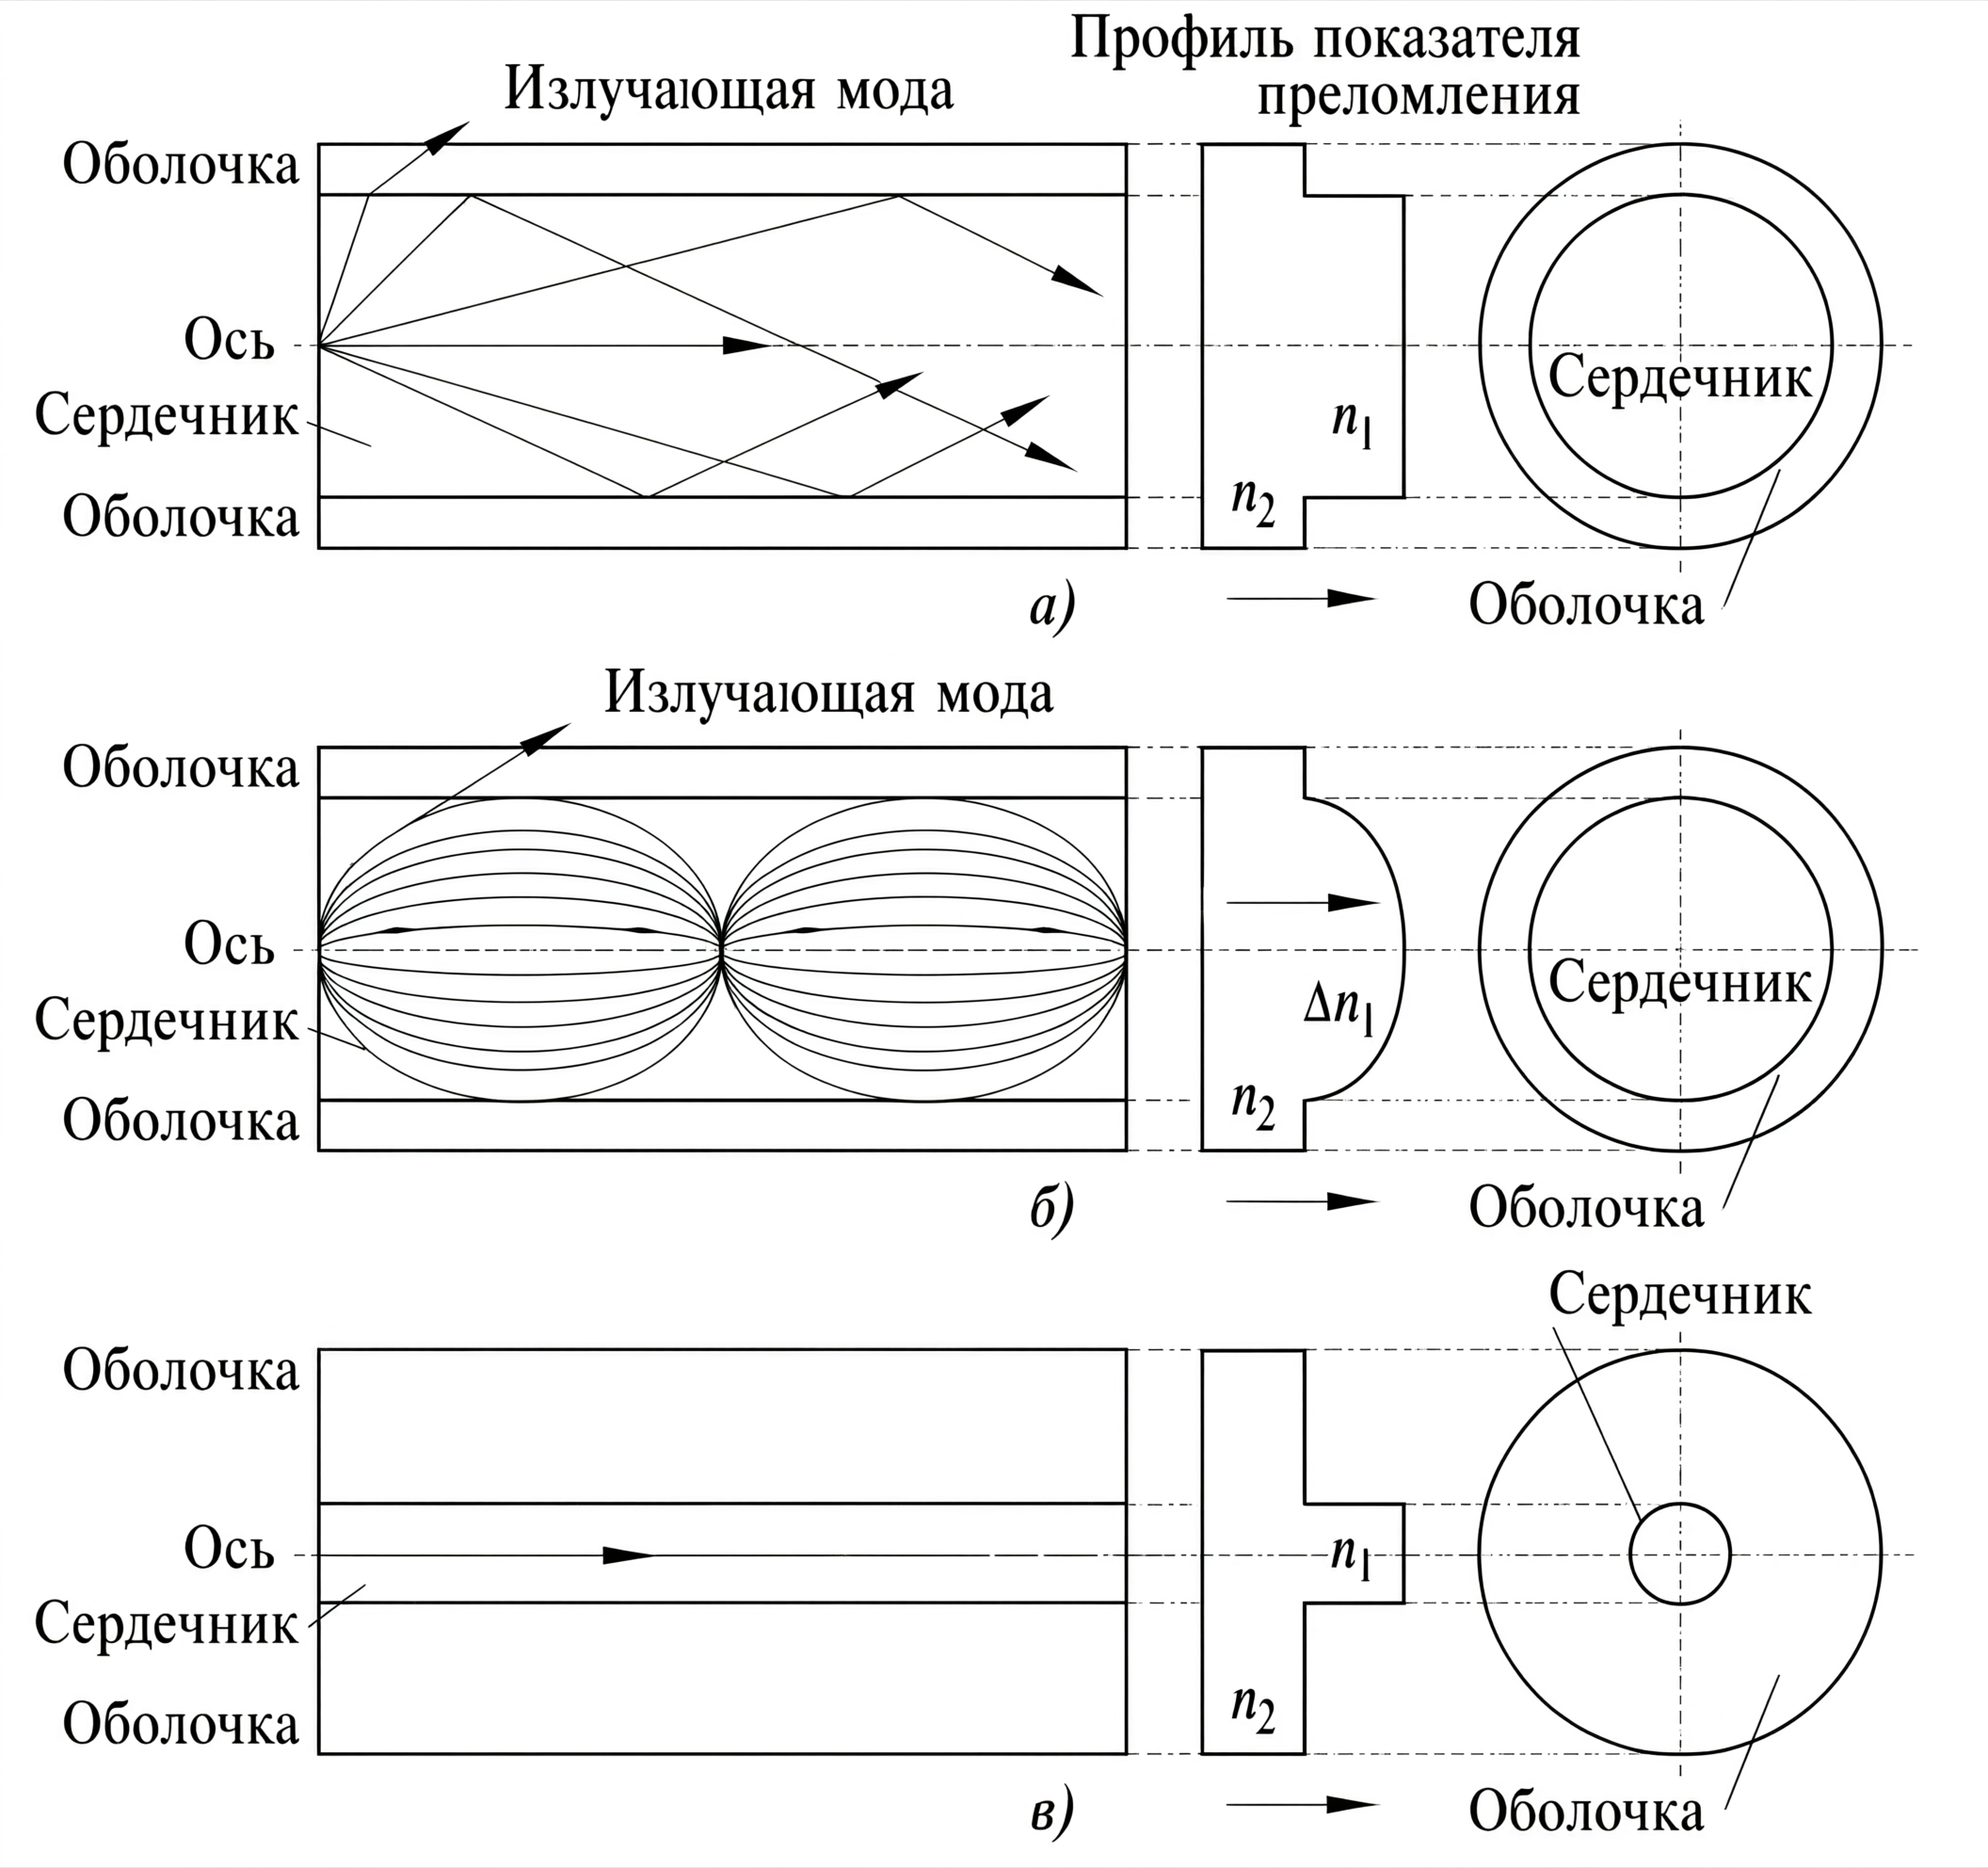
\includegraphics[width=0.8\textwidth]{1790716749199e.png}
    \caption{Профили показателя преломления и модовый состав оптических волокон:
    а~--- многомодовое со ступенчатым профилем;
    б~--- многомодовое с градиентным профилем;
    в~--- одномодовое~\cite{volokonno2012}}
    \label{fig:tips}
\end{figure}

Величина $\mathrm{NA}$ определяет допустимый угловой диапазон ввода излучения (рисунок~\ref{fig:aprtyr}). Волокна с большим значением $\mathrm{NA}$ обеспечивают эффективный захват расходящихся пучков, однако поддерживают значительное число направляемых мод, что увеличивает межмодовую дисперсию и сужает полосу пропускания. Напротив, волокна с малым $\mathrm{NA}$ характеризуются меньшим числом мод и, соответственно, более широкой рабочей полосой.

\begin{figure}[h]
    \centering
    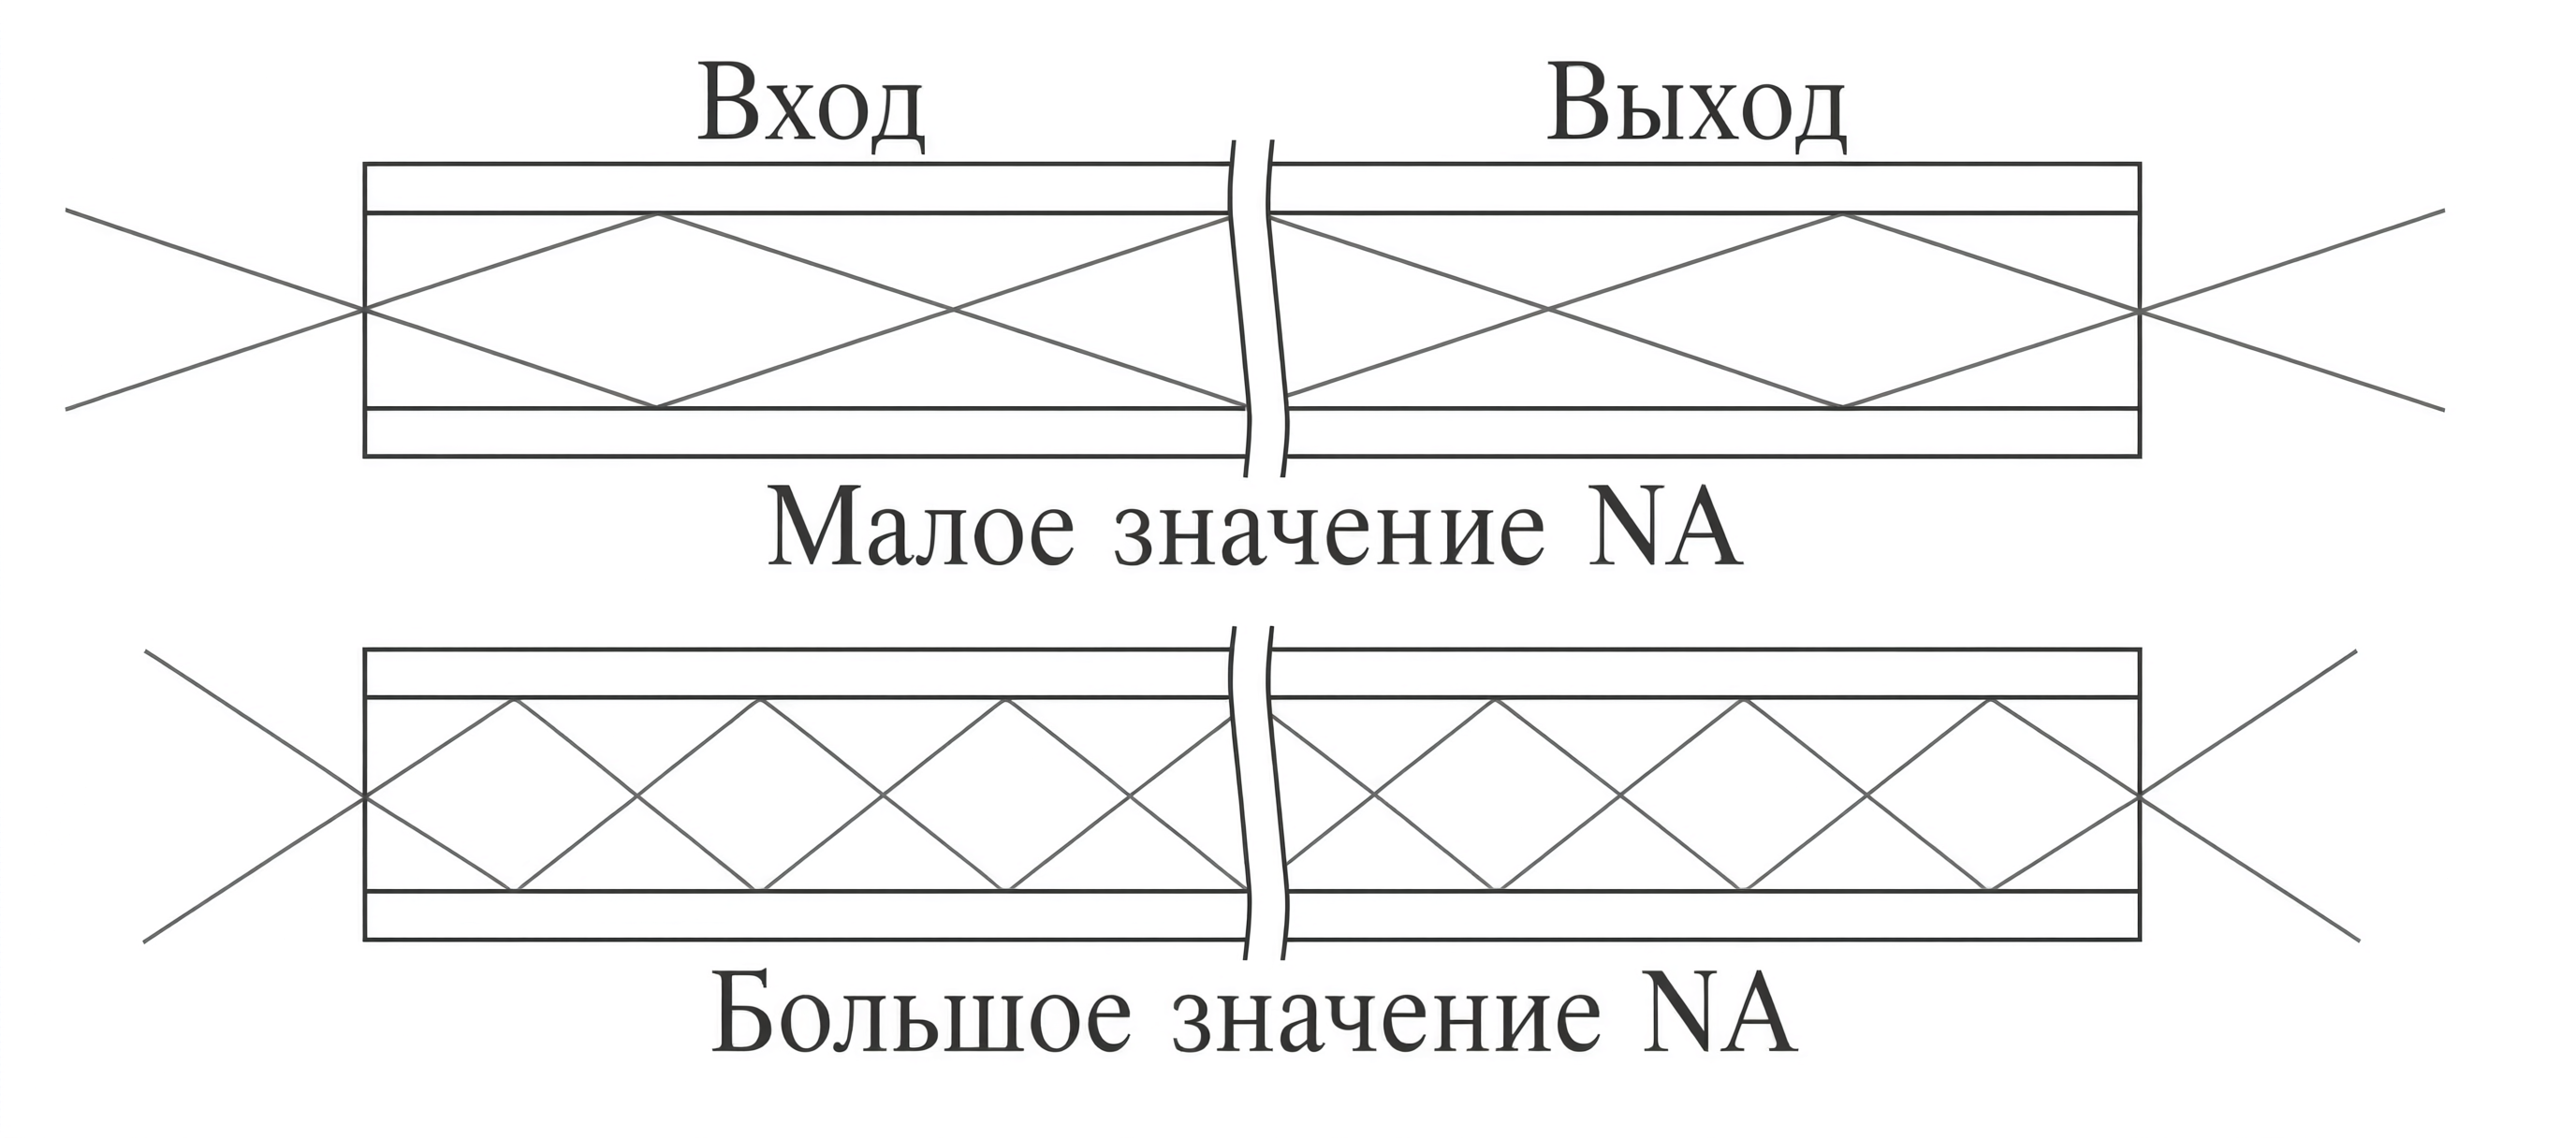
\includegraphics[width=0.8\textwidth]{aperyra.png}
    \caption{Сравнение числовых апертур оптических волокон}
    \label{fig:aprtyr}
\end{figure}

Для одномодовых волокон (типичное значение $\mathrm{NA} \approx 0{,}11$) числовая апертура не является определяющим эксплуатационным параметром, поскольку распространение излучения описывается волновой теорией и не сводится к геометрико-оптической модели полного внутреннего отражения.

Следует учитывать, что эффективное значение $\mathrm{NA}$ уменьшается вдоль длины волокна: моды высоких порядков, распространяющиеся под углами, близкими к критическому, затухают быстрее, в результате чего угловое распределение излучения на выходе сужается относительно входного конуса.

При проектировании волоконно-оптических линий необходимо обеспечивать согласование числовых апертур источника излучения, волокна и фотоприёмника. Рассогласование $\mathrm{NA}$ сопрягаемых компонентов приводит к дополнительным потерям на стыках, пропорциональным квадрату отношения апертур.

\subsubsection{Классификация и характеристики мод оптического волокна}

Присутствие оптической оболочки определяет граничные условия распространения электромагнитных волн в оптическом волокне (ОВ). В зависимости от условий отражения на границе раздела «сердцевина - оболочка» выделяют три типа мод ~\cite{volokonno2012}:
\begin{enumerate}
    \item \textit{направляемые моды} (моды сердцевины), распространяющиеся вдоль сердцевины за счет многократного полного внутреннего отражения;
    \item \textit{моды оболочки}, распространяющиеся в оболочке за счет отражения от границы «оболочка - внешняя среда»;
    \item \textit{излучаемые моды}, покидающие сердцевину при углах падения, меньших критического.
\end{enumerate}

Наличие поглощающего защитного покрытия ОВ эффективно подавляет моды оболочки, рассеивая их энергию, что исключает перекрестные помехи между соседними волокнами в составе оптического кабеля.

Геометрико-оптическая модель распространения лучей является приближенной и не учитывает волновую природу света. Строгое описание электромагнитного поля в ОВ базируется на решении уравнений Максвелла в цилиндрической системе координат $(r, \varphi, z)$, где ось $z$ совпадает с оптической осью волокна (рисунок~\ref{fig:cilindr}).

\begin{figure}[h]
    \centering
    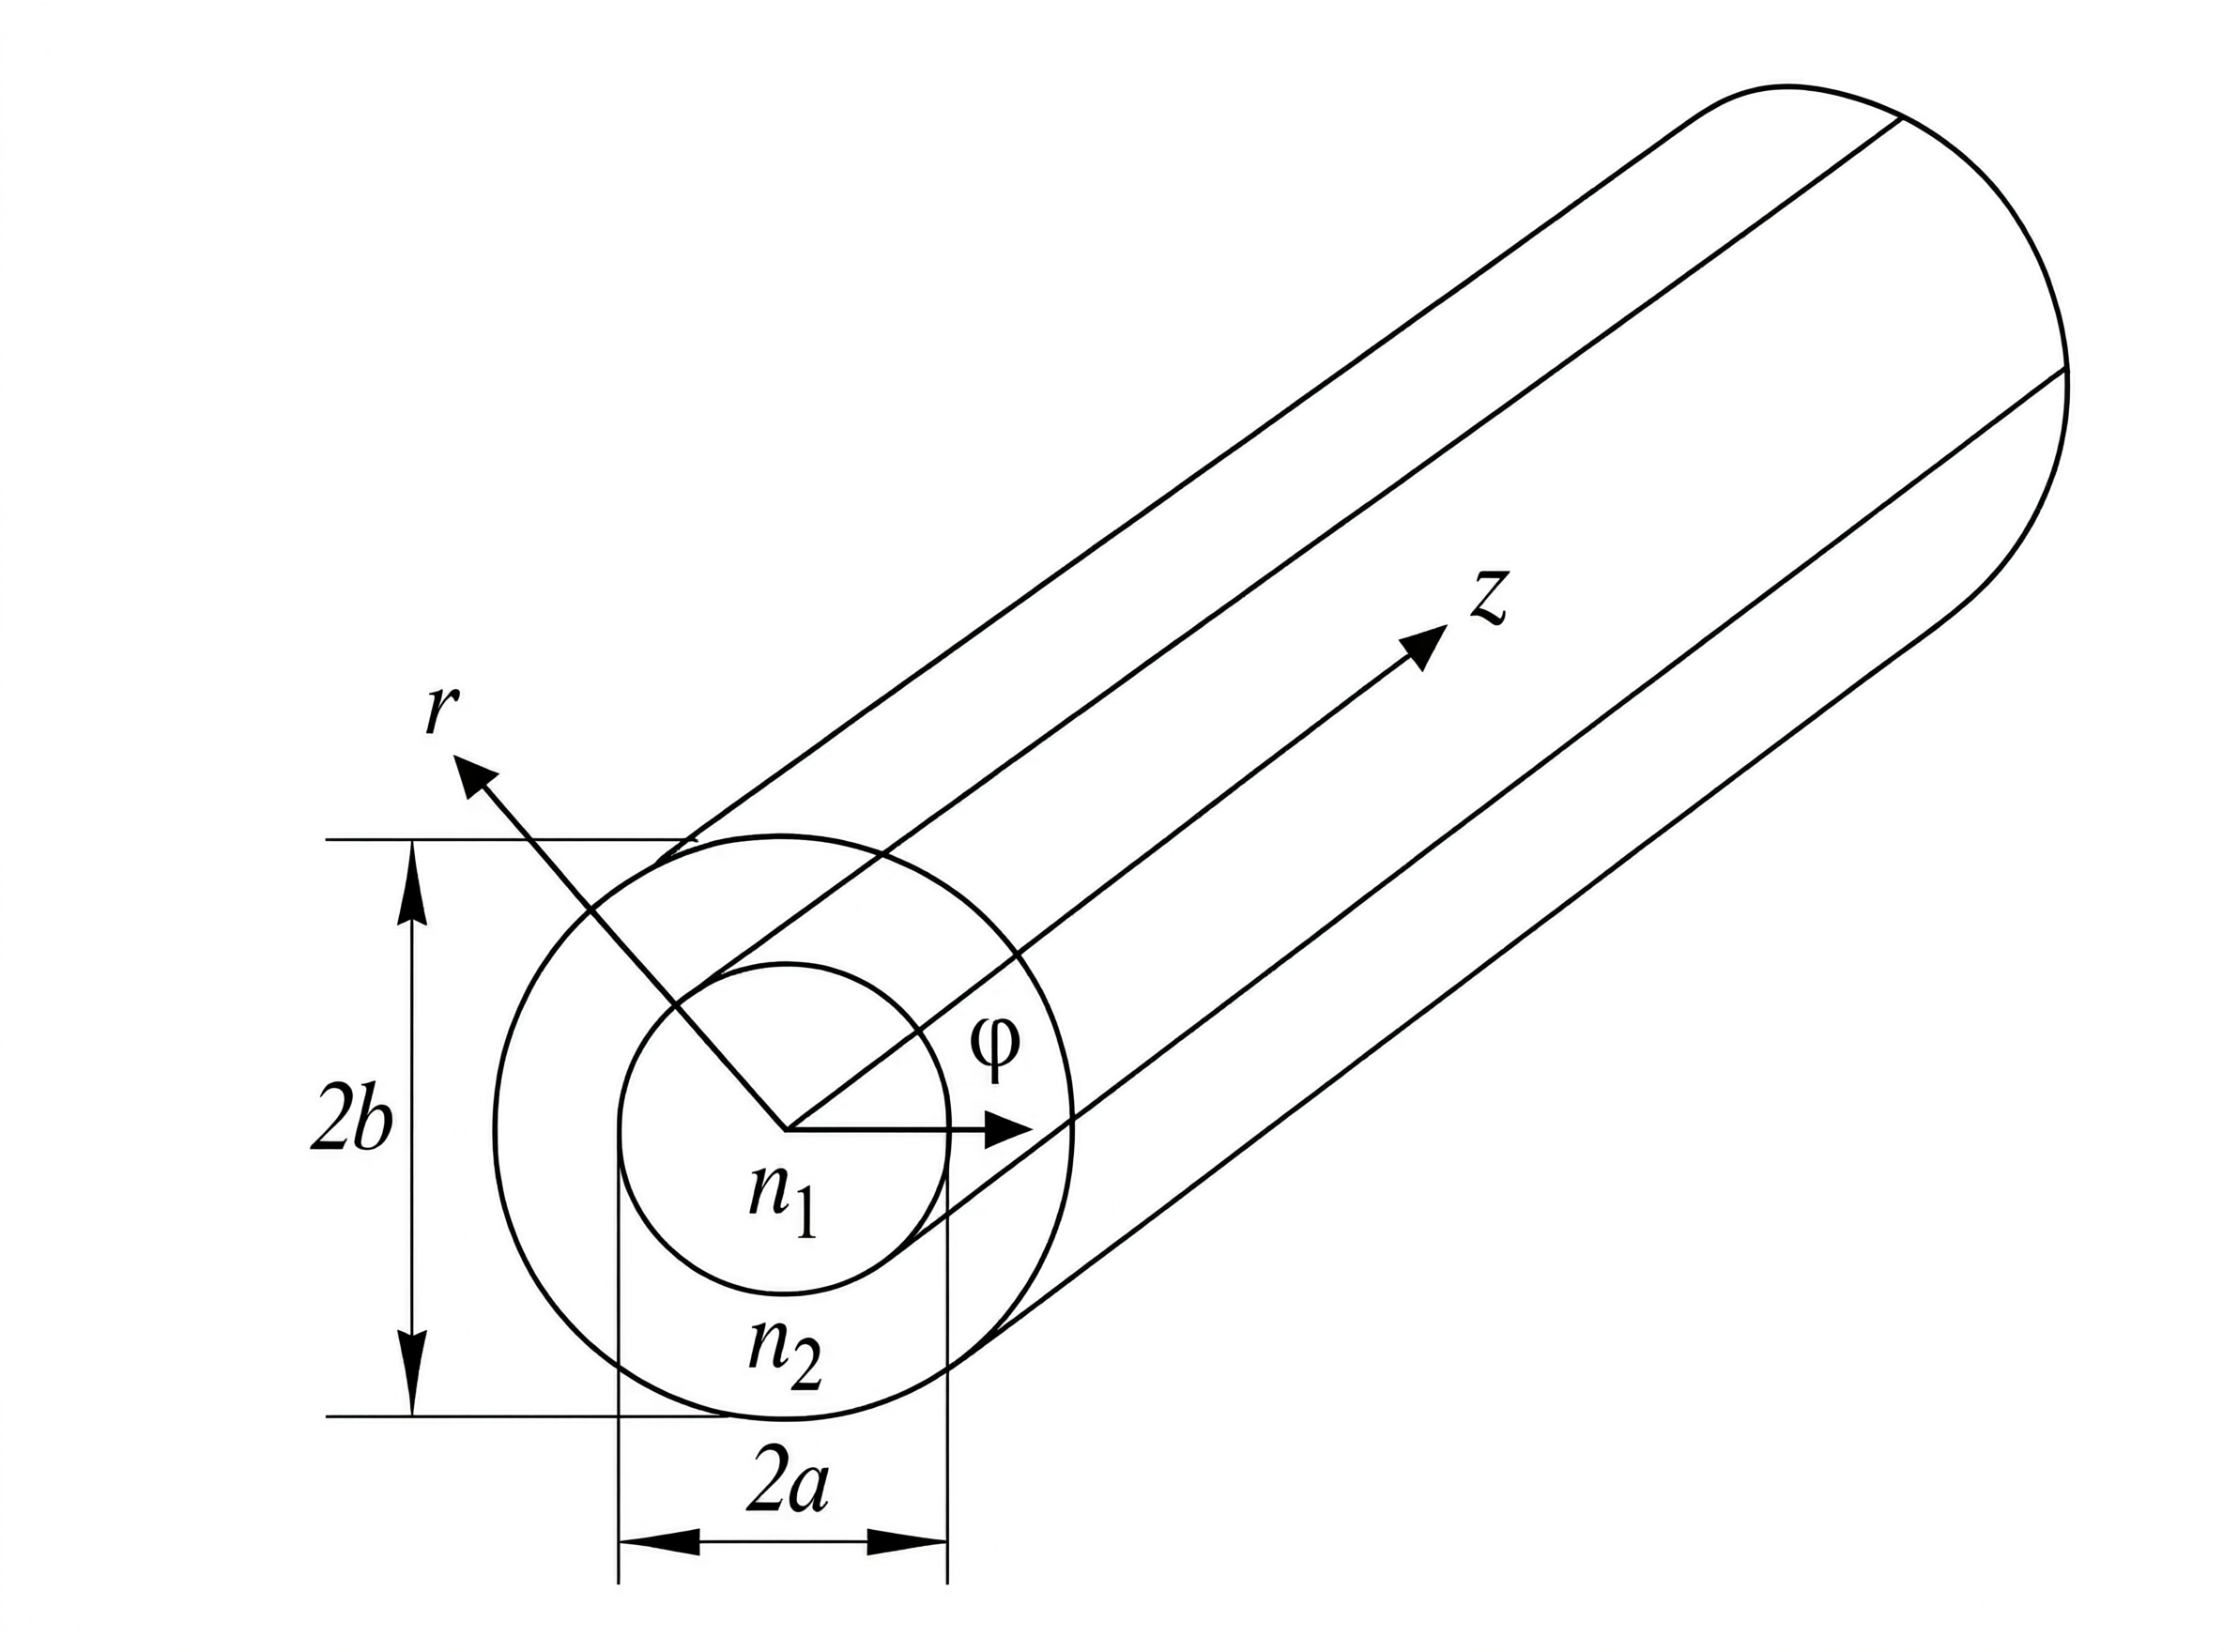
\includegraphics[width=0.8\textwidth]{cilindr.png}
    \caption{Система координат для описания распространения электромагнитных волн в оптическом волокне}
    \label{fig:cilindr}
\end{figure}

Решения уравнений Максвелла позволяют классифицировать направляемые моды по симметрии электромагнитного поля относительно азимутального угла $\varphi$ ~\cite{volokonno2012}:
\begin{enumerate}
    \item \textit{симметричные моды}, не зависящие от $\varphi$. Подразделяются на:
    \begin{itemize}
        \item[--] поперечно-магнитная ($TM$-моды), для которых продольная составляющая электрического поля $E_z \neq 0$, а магнитного $H_z = 0$;
        \item[--] поперечно-электрическая ($TE$-моды), для которых $E_z = 0$, $H_z \neq 0$;
    \end{itemize}
    \item \textit{несимметричные (гибридные) моды}, зависящие от $\varphi$, у которых обе продольные составляющие отличны от нуля ($E_z \neq 0$ и $H_z \neq 0$). В зависимости от преобладающей продольной составляющей их обозначают как $HE$-моды или $EH$-моды.
\end{enumerate}

Структура поля каждой моды однозначно определяется парой индексов $(m, n)$, где:
\begin{enumerate}
    \item[--] $m$ ($m = 0, 1, 2, \dots$) - азимутальный индекс, определяющий периодичность изменения поля по углу $\varphi$;
    \item[--] $n$ ($n = 1, 2, 3, \dots$) - радиальный индекс, определяющий число экстремумов поля вдоль радиуса $r$.
\end{enumerate}
Полное обозначение моды записывается как $HE_{mn}$ или $EH_{mn}$.

Общее число направляемых мод $N$ в многомодовом волокне со ступенчатым профилем показателя преломления оценивается через нормированную частоту $V$ ~\cite{volokonno2012}:
\begin{equation}
    N \approx \frac{V^2}{2},
    \label{eq:N_modes}
\end{equation}
где нормированная частота $V$ определяется выражением ~\cite{velichansky2007}:
\begin{equation}
    V = \frac{2\pi a}{\lambda} \sqrt{n_1^2 - n_2^2} = \frac{2\pi a}{\lambda} \mathrm{NA}.
    \label{eq:V_number}
\end{equation}
Здесь $a$ - радиус сердцевины, $\lambda$ - длина волны излучения в вакууме, $n_1$ и $n_2$ - показатели преломления сердцевины и оболочки соответственно, $\mathrm{NA}$ - числовая апертура.

\subsubsection{Критическая частота }

Изменение нормированной частоты $V$, определяемой соотношением структурных параметров волокна и длины волны излучения, приводит к изменению числа направляемых мод. Появление или исчезновение каждой моды происходит при строго определённых значениях $V$, называемых \textit{критическими частотами} и обозначаемых $V_{mn}$.

Условие
\begin{equation}
    V = V_{mn} \quad (m = 0, 1, 2, \dots; \quad n = 1, 2, 3, \dots)
    \label{eq:Vmn}
\end{equation}
определяет границу существования направляемой моды. В рамках геометрико-оптического приближения данному условию соответствует угол скольжения $\varphi = \varphi_\text{кр}$. При $V > V_{mn}$ ($\varphi > \varphi_\text{кр}$) выполняется условие полного внутреннего отражения, и мода распространяется в сердцевине; при $V < V_{mn}$ мода переходит в разряд излучаемых.

Особое положение занимает мода $HE_{11}$, для которой критическая частота $V_{11} = 0$. Поскольку условие $V > 0$ выполняется всегда, данная мода распространяется в волокне при любых структурных параметрах и длинах волн. Она называется \textit{основной} (фундаментальной). Все остальные моды классифицируются как \textit{высшие}.

Наибольший практический интерес представляет \textit{одномодовый режим}, при котором в волокне распространяется только основная мода. Условие одномодового режима записывается как:
\begin{equation}
    V = \frac{2\pi a}{\lambda}\sqrt{n_1^2 - n_2^2} = \frac{2\pi a}{\lambda}\mathrm{NA} \leq 2{,}405.
    \label{eq:single_mode}
\end{equation}

В силу азимутальной симметрии идеального волокна основная мода обладает поляризационным вырождением: в нём одновременно распространяются две ортогональные поляризационные моды с идентичными характеристиками. Нарушение симметрии (например, эллиптичность сердцевины или механические напряжения) снимает это вырождение, приводя к возникновению собственного двойного лучепреломления и поляризационной модовой дисперсии.

Фазовая скорость $v_\text{ф}$ направляемых мод определяется из решения дисперсионных уравнений. На рисунке~\ref{fig:dispersionnsqhar} представлены дисперсионные характеристики, связывающие нормированную фазовую скорость $c/v_\text{ф}$ с нормированной частотой $V$ для основной и высших мод.

Значения фазовой скорости для всех направляемых мод строго ограничены пределами:
\begin{equation}
    \frac{c}{n_1} \leq v_\text{ф} \leq \frac{c}{n_2} \quad \Leftrightarrow \quad n_2 \leq \frac{c}{v_\text{ф}} \leq n_1,
    \label{eq:phase_velocity}
\end{equation}
где $c$ - скорость света в вакууме.

\begin{figure}[h]
    \centering
    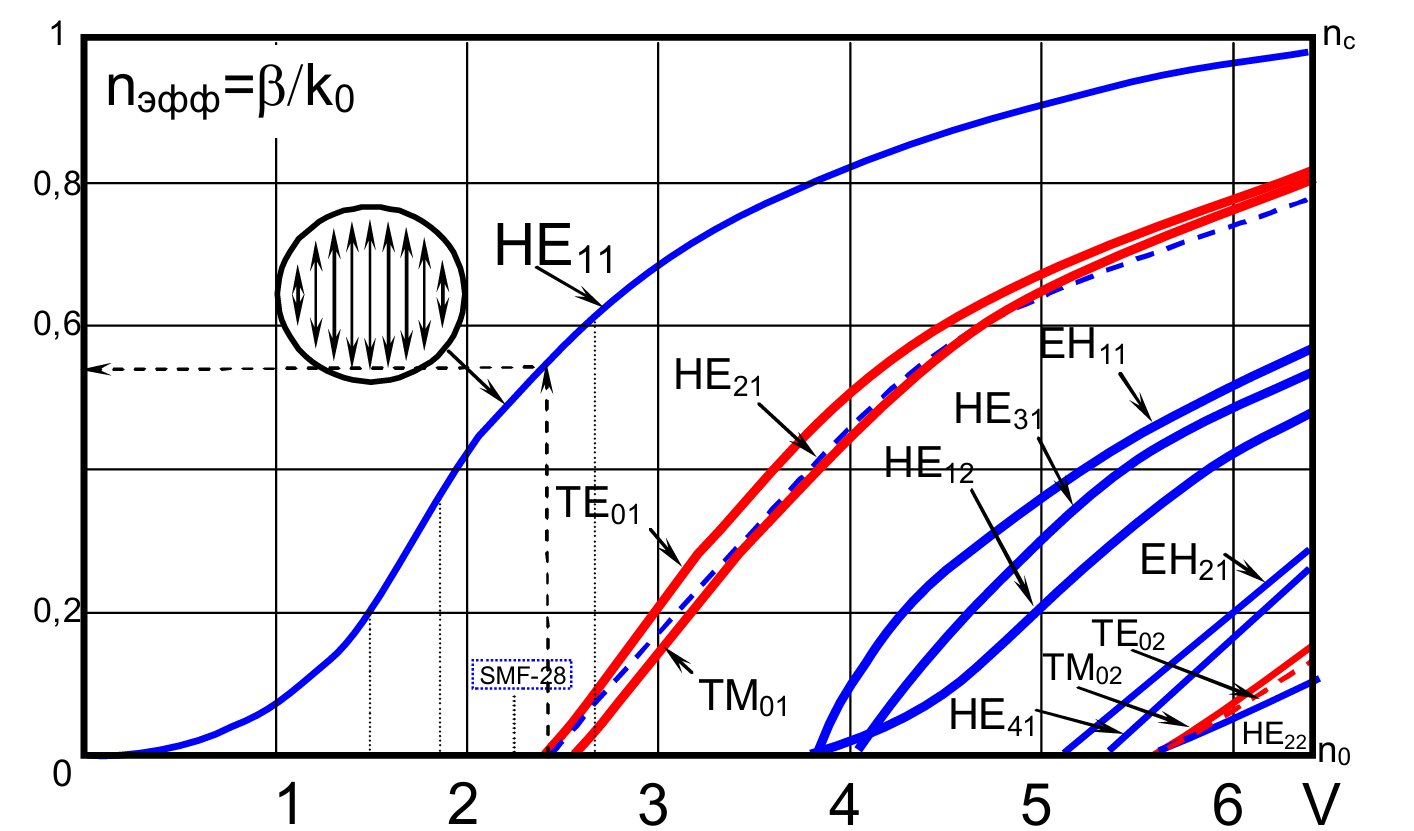
\includegraphics[width=0.8\textwidth]{dispersionnsq harakter.png}
    \caption{ Зависимость нормированной постоянной распространения от приведенного диаметра диэлектрического волновода для основной моды $HE_{11}$ и для низших мод~\cite{velichansky2007}}
    \label{fig:dispersionnsqhar}
\end{figure}

При изгибах оптического волокна условия полного внутреннего отражения для высших мод нарушаются, что приводит к их излучению в оболочку.

\subsection{Параметры оптических волокон}

\subsubsection{Коэффициент затухания оптического сигнала}

Затухание оптического сигнала в оптическом кабеле (ОК) обусловлено собственными потерями мощности в изолированном прямолинейном оптическом волокне (ОВ) и дополнительными (кабельными) потерями, возникающими при сборке ОВ в кабель. Таким образом, суммарный коэффициент затухания ОВ в составе кабеля $\alpha$ определяется выражением:
\begin{equation}
    \alpha = \alpha_\text{с} + \alpha_\text{доп},
    \label{eq:alpha_total}
\end{equation}
где $\alpha_\text{с}$ - собственные потери; $\alpha_\text{доп}$ - дополнительные потери.

\subsubsubsection{Собственные потери}

Собственные потери мощности обусловлены преимущественно поглощением энергии в материале ОВ и рассеянием излучения. Потери на поглощение включают собственное поглощение материала (в ультрафиолетовой и инфракрасной областях) и поглощение на примесях.

Примесные центры поглощают излучение на характерных для них длинах волн. Даже незначительные концентрации примесей формируют выраженные пики на спектральной кривой потерь. Наиболее существенное влияние оказывают ионы гидроксильных групп (OH$^-$). Соответствующий «водный пик» в области $\lambda \approx 1{,}39$~мкм присутствует во всех современных ОВ, изготовленных по стандартной промышленной технологии, вследствие чего данный спектральный диапазон практически не используется для передачи сигналов.

Собственные потери на поглощение экспоненциально возрастают в инфракрасной области. При $\lambda > 1{,}8$~мкм стандартное кварцевое ОВ становится непрозрачным.

Потери на рассеяние вызваны микроскопическими флуктуациями показателя преломления (неоднородностями), неизбежно возникающими при изготовлении ОВ. Данный механизм, известный как рэлеевское рассеяние, подчиняется закону $\lambda^{-4}$.

В длинноволновой области спектра (1,3-1,6~мкм) наблюдаются два минимума потерь (окна прозрачности). По сравнению с $\lambda = 0{,}85$~мкм (первое окно прозрачности), собственные потери при $\lambda = 1{,}3$~мкм (второе окно) снижаются примерно в 3~раза, а при $\lambda = 1{,}55$~мкм (третье окно) - в 8--10~раз.

Спектральная зависимость потерь и положение окон прозрачности в кварцевых ОВ представлены на рисунке~\ref{fig:spectpoteri}.

\begin{figure}[h]
    \centering
    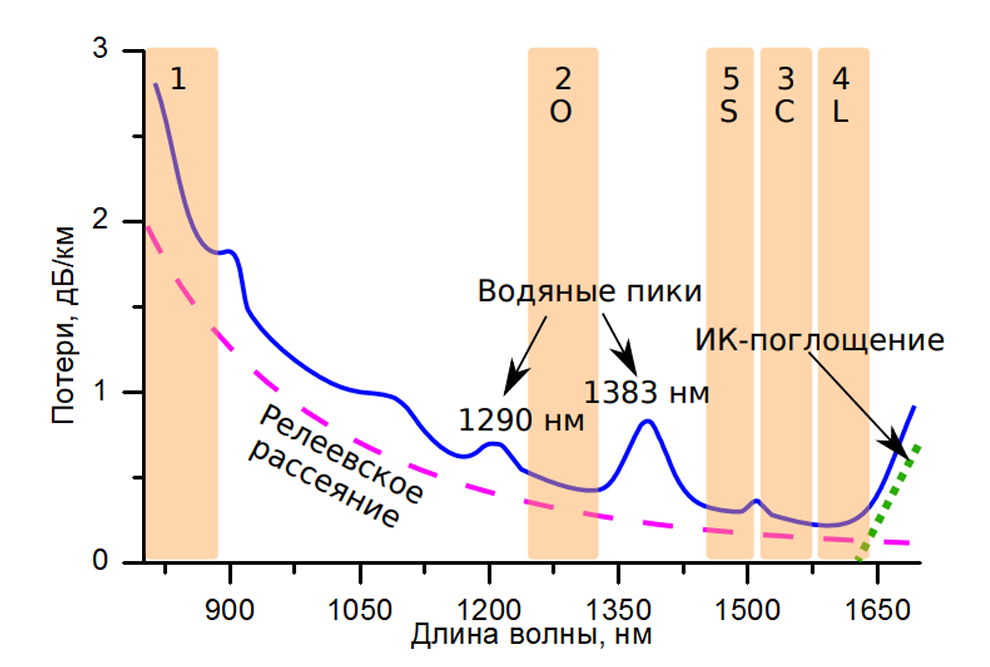
\includegraphics[width=0.8\textwidth]{spectr poteri.png}
    \caption{Спектр потерь и положение окон прозрачности в кварцевых оптических волокнах ~\cite{volokonno2012}}
    \label{fig:spectpoteri}
\end{figure}

\subsubsubsection{Дополнительные (кабельные) потери}

Дополнительные (кабельные) потери возникают при нанесении на ОВ защитного полимерного покрытия и в результате механических деформаций волокна при сборке ОК.

Защитное покрытие повышает механическую надежность ОВ и снижает перекрестные помехи. Увеличение толщины оболочки ОВ уменьшает проникновение поля направляемых мод в покрытие, снижая дополнительные потери, однако ухудшает гибкость и увеличивает стоимость. Для многомодовых ОВ диаметр оболочки выбирают в 2,0-2,5~раза больше диаметра сердцевины (потери в покрытии $\le 0{,}1$~дБ/км). Для одномодовых ОВ, вследствие значительного проникновения поля основной моды в оболочку, толщина оболочки должна превышать радиус сердцевины в 10 и более раз.

Деформации ОВ при изготовлении кабеля (микроизгибы, скрутка, сжатие) формируют вторую составляющую дополнительных потерь. При оптимальном выборе материалов и конструкции ОК эти потери составляют не более 20~\% от суммарных.

В процессе строительства и эксплуатации возникают эксплуатационные потери, связанные с макроизгибами ОВ и постепенной деградацией материала. Потери на макроизгибах обусловлены преобразованием направляемых мод в моды излучения (рисунок~\ref{fig:izgib}~а). Они критически возрастают при уменьшении радиуса изгиба до нескольких сантиметров. В связи с этим технические условия на ОК строго регламентируют минимально допустимый радиус изгиба. Основной причиной постепенного увеличения собственных потерь со временем является проникновение влаги в ОК, что приводит к помутнению стекла и росту микротрещин. Для предотвращения этого применяют влагозащитные оболочки и гидрофобный заполнитель.

\begin{figure}[h]
    \centering
    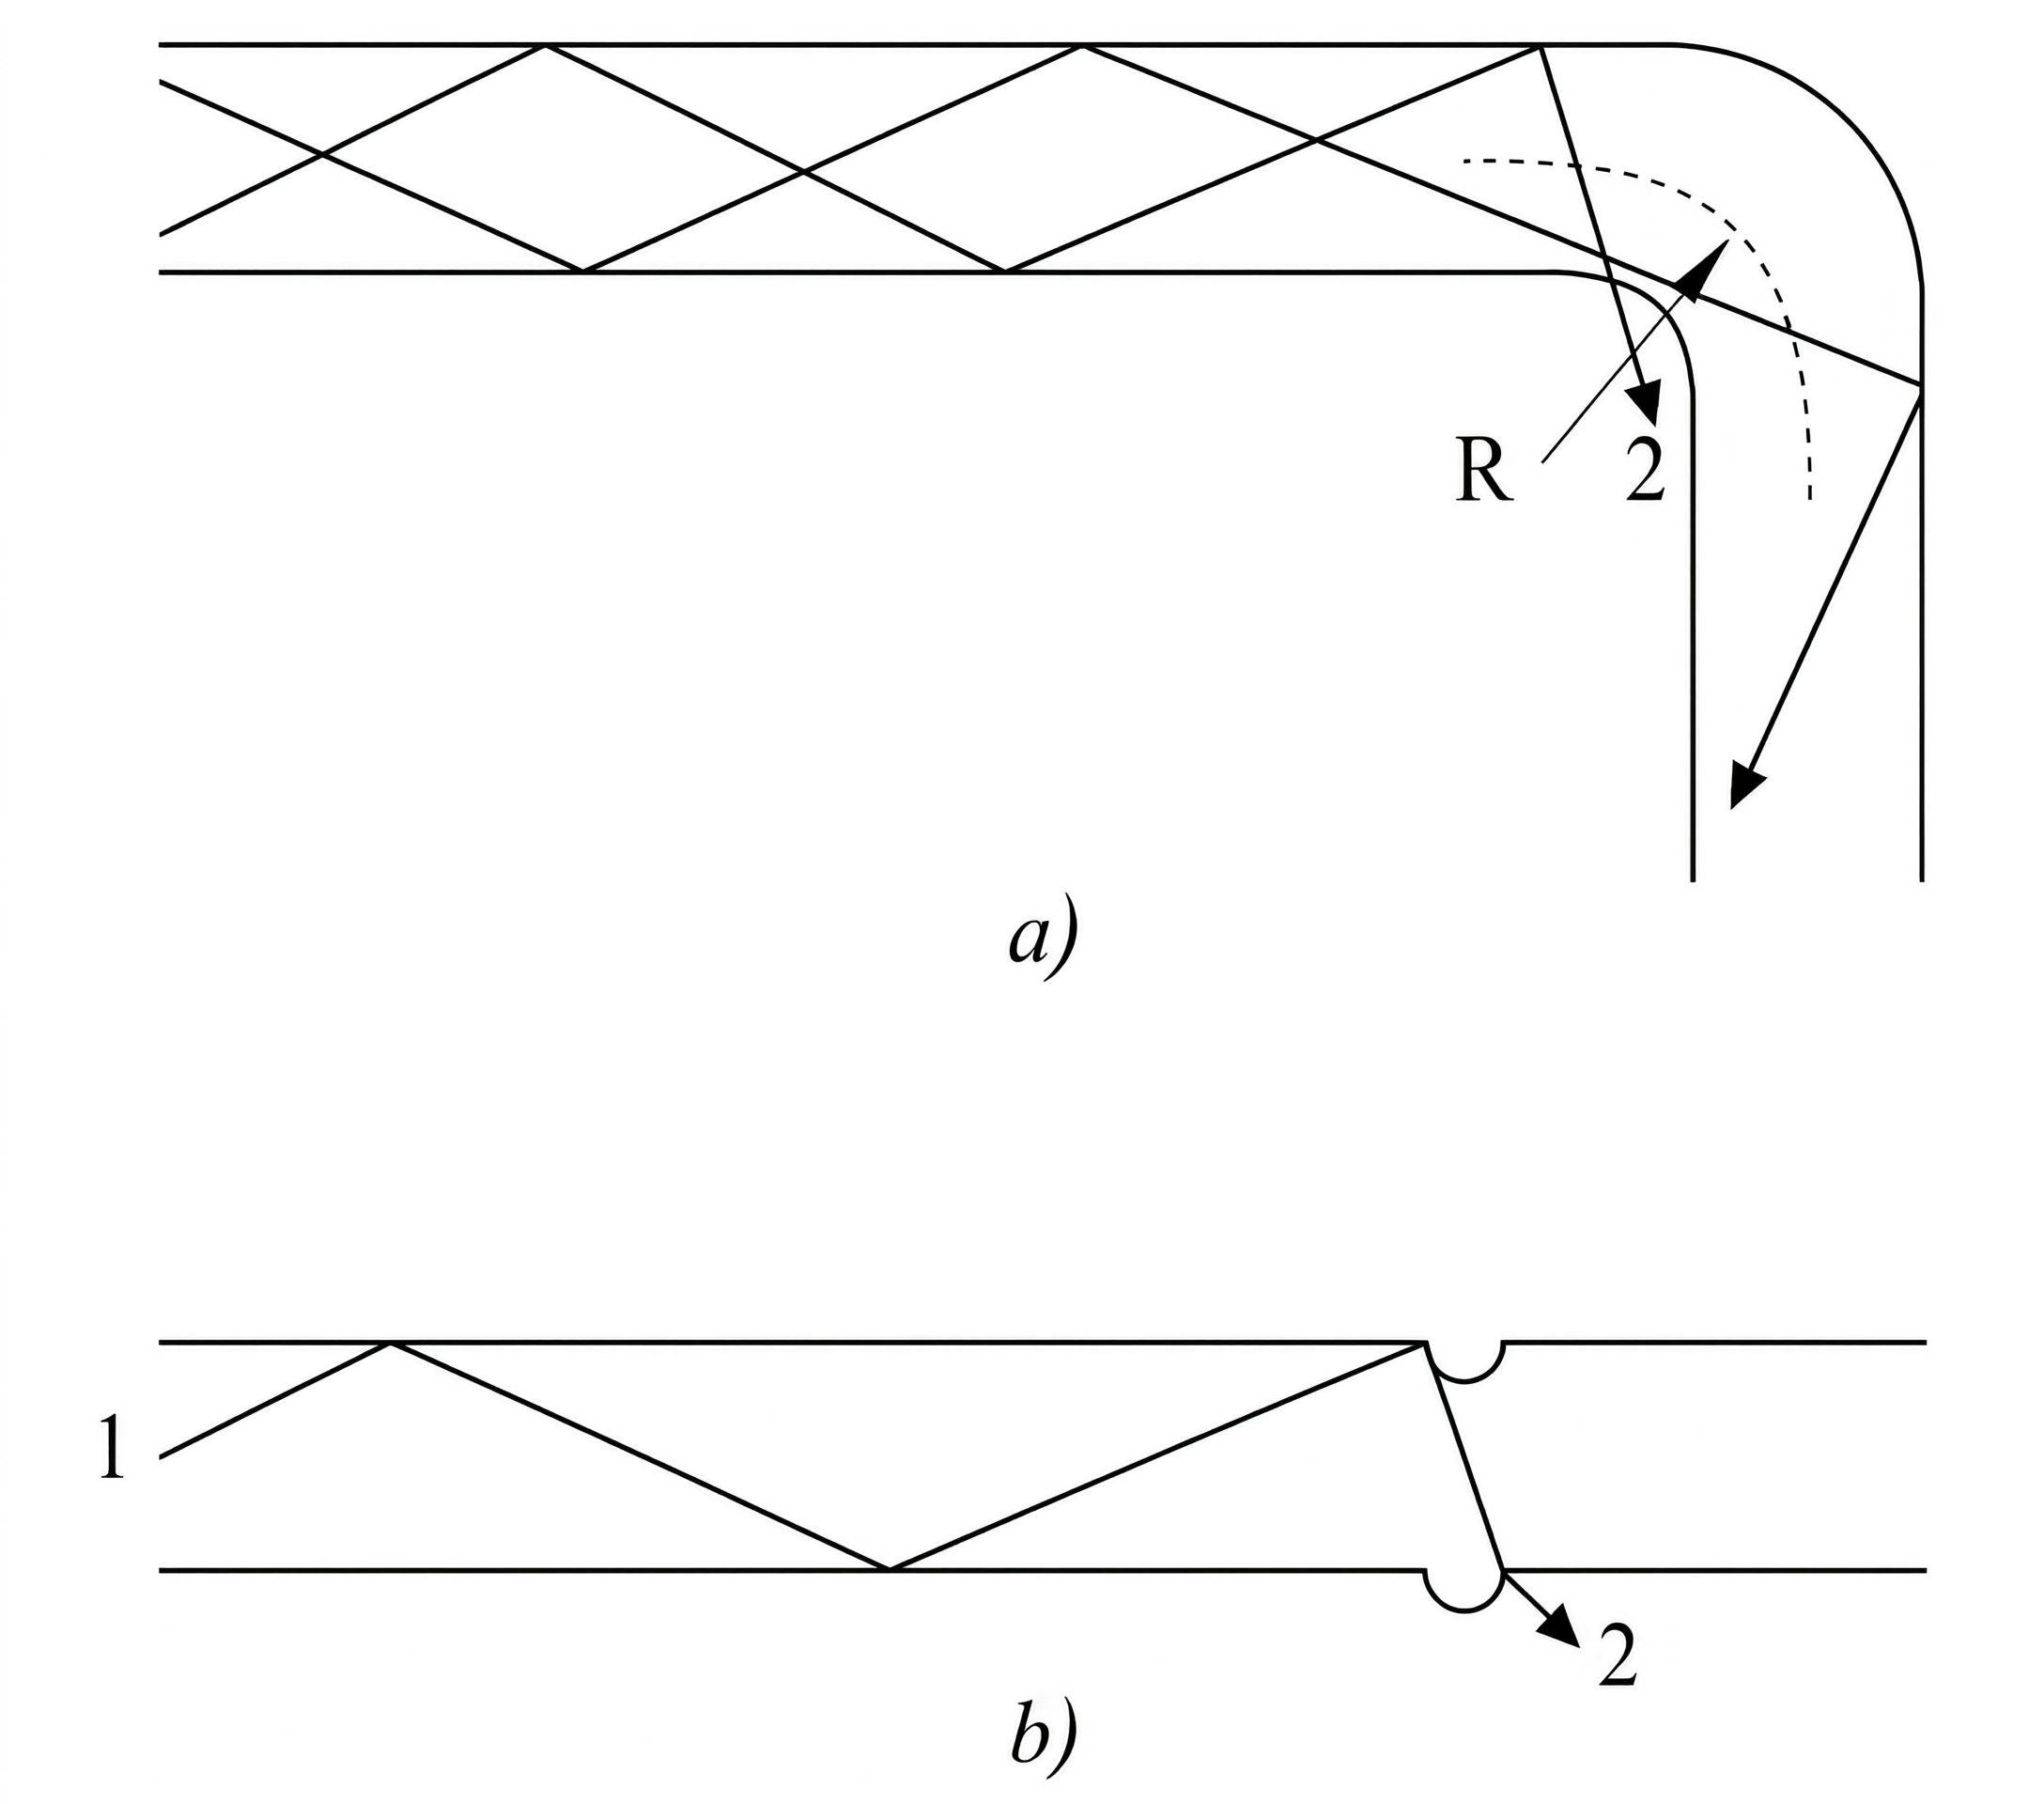
\includegraphics[width=0.6\textwidth]{izgib.png}
    \caption{Потери на изгибах оптического волокна:
    а~--- на макроизгибе;
    б~--- на микроизгибе}
    \label{fig:izgib}
\end{figure}

Макроизгибы представляют собой макроскопические отклонения оси ОВ от прямой, возникающие при намотке кабеля на барабан, прокладке и монтаже. На рисунке~\ref{fig:izgib}~а показано преобразование направляемой моды~1 в вытекающую моду~2.

Микроизгибы ~\cite{volokonno2012} - это случайные микроскопические искривления оси волокна на единицы микрометров (рисунок~\ref{fig:izgib}~б), вызванные локализованными поперечными нагрузками. Они возникают из-за деформаций при изготовлении и прокладке, а также вследствие температурных расширений материалов кабеля. Чувствительность ОВ к микроизгибам зависит от разности показателей преломления сердцевины и оболочки, а также их геометрических размеров. Микроизгибы приводят к значительным потерям на излучение и межмодовому взаимодействию.

\subsubsection{Релеевское рассеяние}

Релеевское рассеяние представляет собой упругое рассеяние электромагнитного излучения на микронеоднородностях среды, характерный размер которых существенно меньше длины волны $\lambda$. В кварцевых оптических волокнах (ОВ) основным механизмом релеевского рассеяния являются флуктуации показателя преломления, обусловленные замороженными термодинамическими флуктуациями плотности материала при его остывании, а также концентрационными флуктуациями, вызванными неравномерным распределением легирующих примесей (рисунок~\ref{fig:reelq}).

\begin{figure}[h]
    \centering
    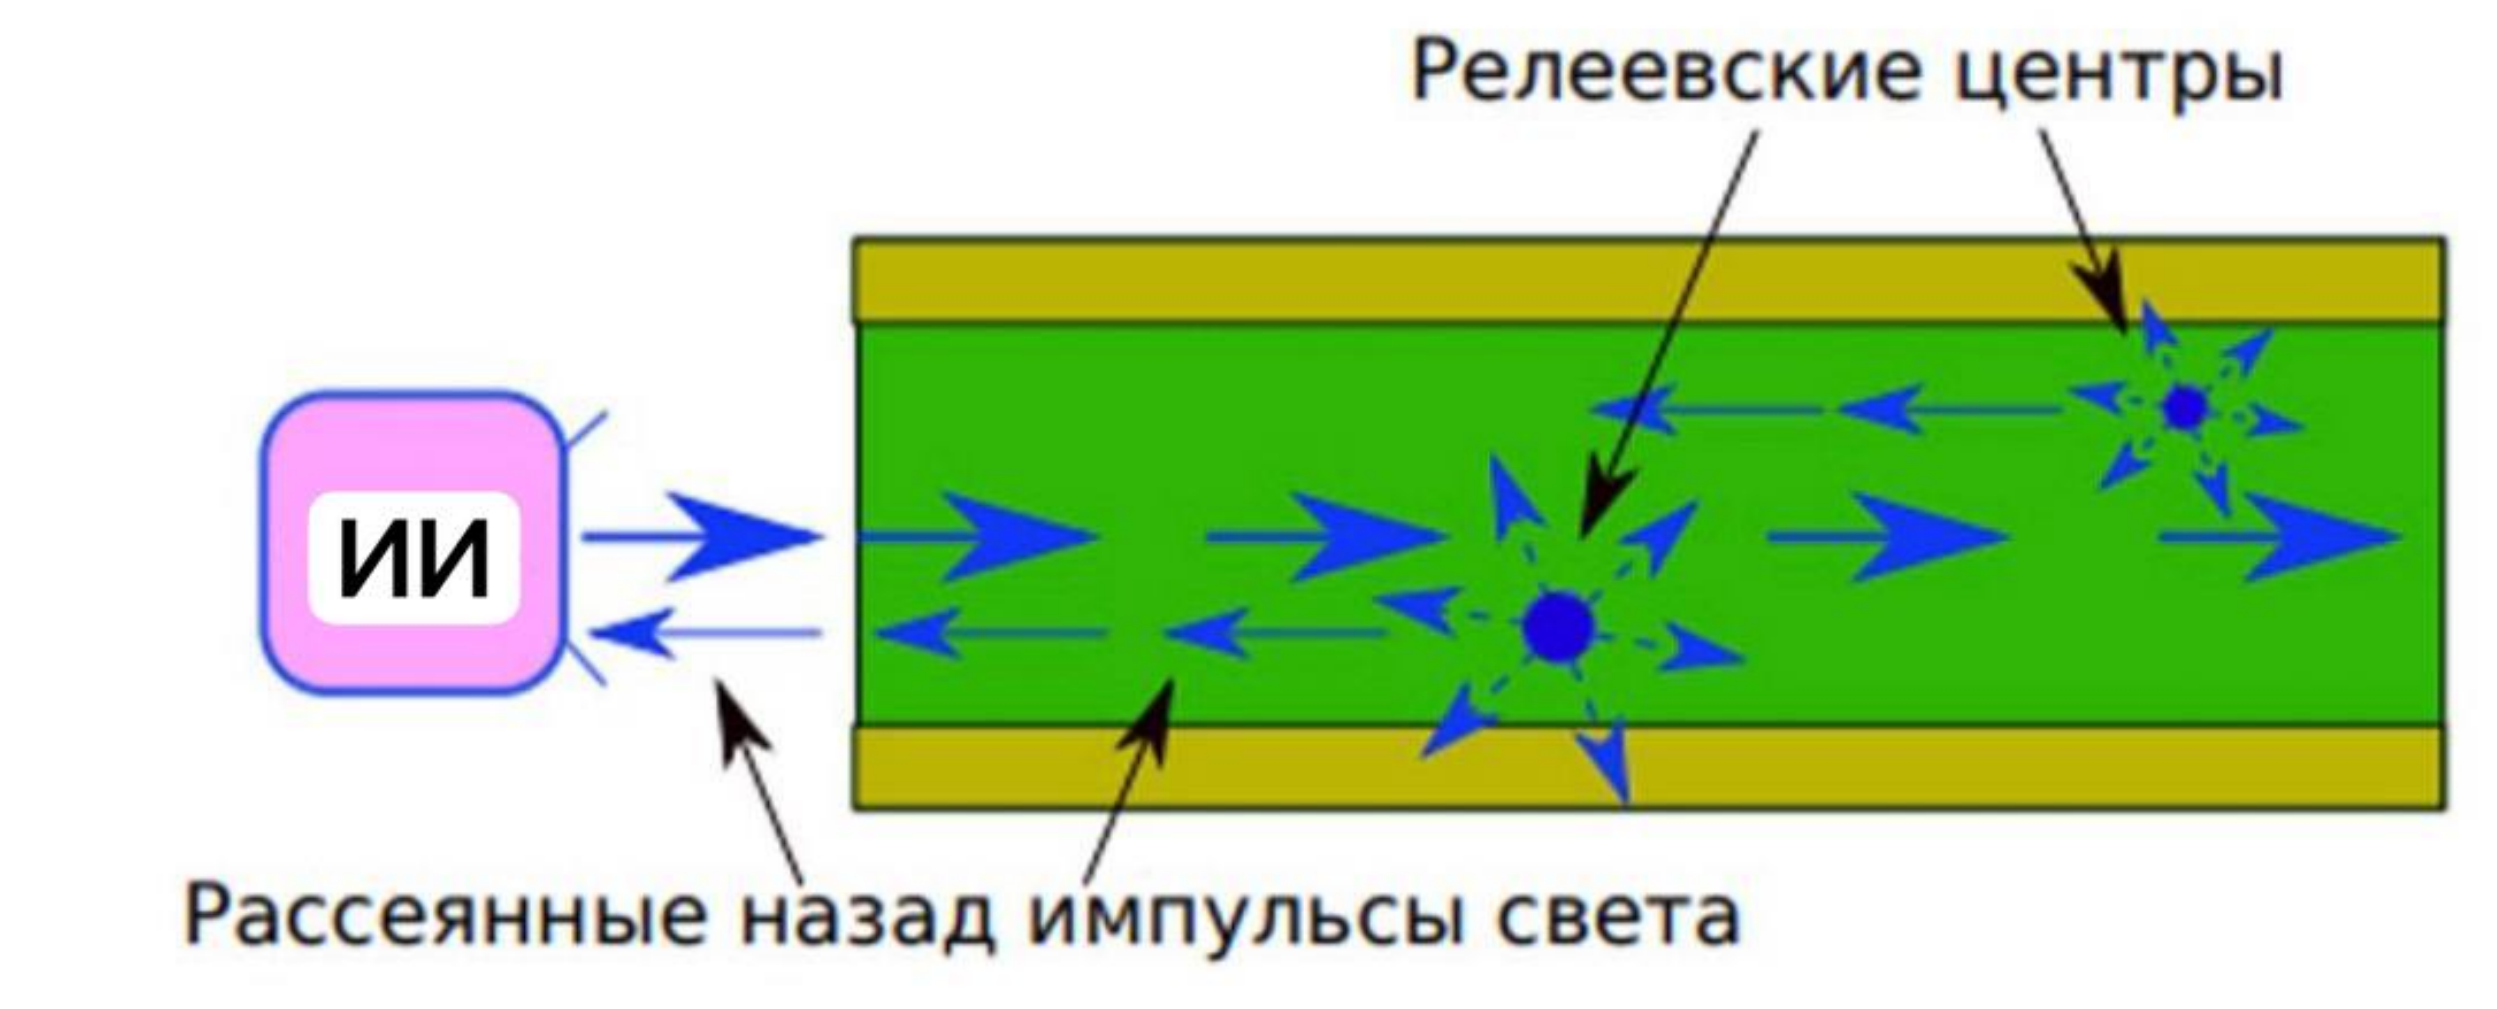
\includegraphics[width=0.8\textwidth]{releeq.png}
    \caption{Релеевское рассеяние в оптическом волокне: ИИ - источник излучения}
    \label{fig:reelq}
\end{figure}

Индикатриса релеевского рассеяния симметрична и охватывает все пространственные углы. Однако в волоконном световоде вдоль оси распространяются лишь те рассеянные фотоны, угол между волновым вектором которых и оптической осью не превышает апертурного угла, определяемого числовой апертурой $\mathrm{NA}$. Остальная часть рассеянной мощности выводится из сердцевины в оболочку и поглощается защитным покрытием.

В отличие от обычного отражения, которое является локализованным эффектом на резкой границе раздела сред, релеевское рассеяние представляет собой протяженный объемный процесс. При таком рассеянии не происходит сохранения формы и длительности оптического импульса, в отличие от зеркального отражения.

Наряду с рэлеевским рассеянием, в оптическом волокне возможен нелинейный процесс - рассеяние Мандельштама–Бриллюэна (РМБ). Оно возникает при распространении в волокне достаточно интенсивного узкополосного излучения (спектр порядка 50-100 МГц), когда продольные упругие колебания микрочастиц стекла, взаимодействуя между собой, формируют бегущую звуковую (акустическую) волну. Кванты таких колебаний - акустические фононы - имеют широкий частотный спектр (до $\approx 10^{13}$~Гц), однако для эффективного возбуждения РМБ необходима высокая спектральная плотность накачки: порядка 10 мВт в полосе 10-50 МГц. Рассеяние света на движущихся акустических волнах сопровождается доплеровским уширением, в результате чего спектр рассеянного излучения расширяется до 300-500 МГц.

\subsubsection{Потери мощности в оптических коннекторах}

Оптические коннекторы предназначены для создания разъемных механических соединений волоконно-оптических линий связи. Основным элементом коннектора является ферула - высокоточный направляющий наконечник, фиксирующий оптическое волокно.

Вносимые потери мощности в коннекторном соединении обусловлены геометрическим рассогласованием световодов (осевым, поперечным и угловым), наличием воздушного зазора между торцами, а также дефектами и загрязнениями поверхности. Для минимизации воздушного зазора и снижения обратных потерь применяют специальные профили шлифовки торцов ферул.

Наиболее распространены цилиндрические керамические ферулы диаметром 2{,}5~мм (стандарты FC, SC, ST) и 1{,}25~мм (стандарт LC). Плоская шлифовка обеспечивает базовое соединение, однако выпуклая сферическая полировка (радиус кривизны 10--15~мм) гарантирует физический контакт сердцевин и существенно снижает обратные потери. Для применений, критичных к паразитным отражениям, используется угловая полировка торца под углом 8°(рисунок~\ref{fig:optical_connect}). Контроль качества и чистоты торцов осуществляется с помощью микроскопов с увеличением в сотни раз .

\begin{figure}[h]
    \centering
    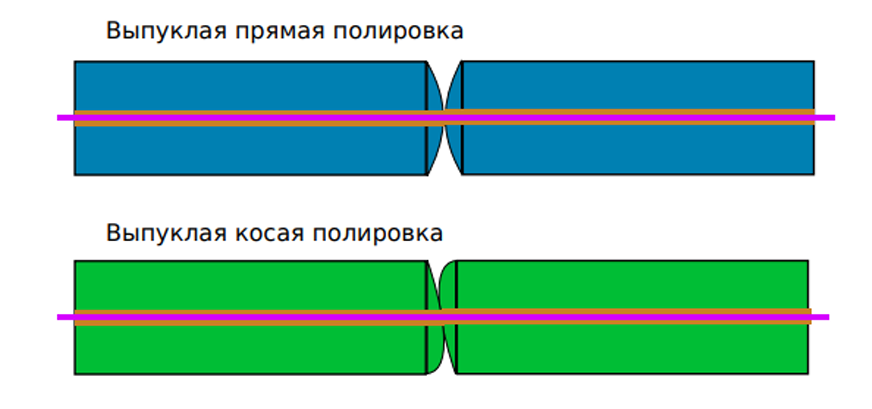
\includegraphics[width=0.8\textwidth]{connect.png}
    \caption{Типы полировки оптических наконечников}
    \label{fig:optical_connect}
\end{figure}

Для точного центрирования ферул при стыковке используется адаптер (оптическая розетка)~\cite{volokonno2012} - механический интерфейс, обеспечивающий жесткую фиксацию и соосное сопряжение коннекторов. Конструкция адаптера и коннектора определяет допустимые допуски на смещение, что напрямую влияет на итоговые вносимые потери оптического тракта.

\subsubsection{Дисперсия оптического сигнала}

Наряду с коэффициентом затухания, важнейшей характеристикой оптического волокна (ОВ) является дисперсия, определяющая его информационную пропускную способность.

Дисперсия в волокне обусловлена различием групповых задержек спектральных или модовых составляющих сигнала. Она может вызывать уширение оптического импульса (рисунок~\ref{fig:rasprostr}). При описании уширения свёрткой входного профиля с распределением задержек их временные дисперсии складываются. Для гауссовых профилей ширина на полувысоте пропорциональна среднеквадратичной ширине с одинаковым множителем. Тогда вклад уширения можно выразить через ширины импульса на выходе ($\tau_\text{вых}$) и входе ($\tau_\text{вх}$) волокна
\begin{equation}
    \tau = \sqrt{\tau_\text{вых}^2 - \tau_\text{вх}^2},
    \label{eq:tau_total}
\end{equation}
Для произвольных форм импульса ширины на полувысоте зависят от профиля сигнала.

Дисперсия ограничивает частотный диапазон и максимальную дальность передачи сигналов, поскольку с увеличением длины линии накопление временного уширения возрастает. В общем случае дисперсия обусловлена различием скоростей распространения направляемых мод, направляющими свойствами волноводной структуры и дисперсией материала. Исходя из этого, выделяют межмодовую и хроматическую (внутримодовую) дисперсию.

\begin{figure}[h]
    \centering
    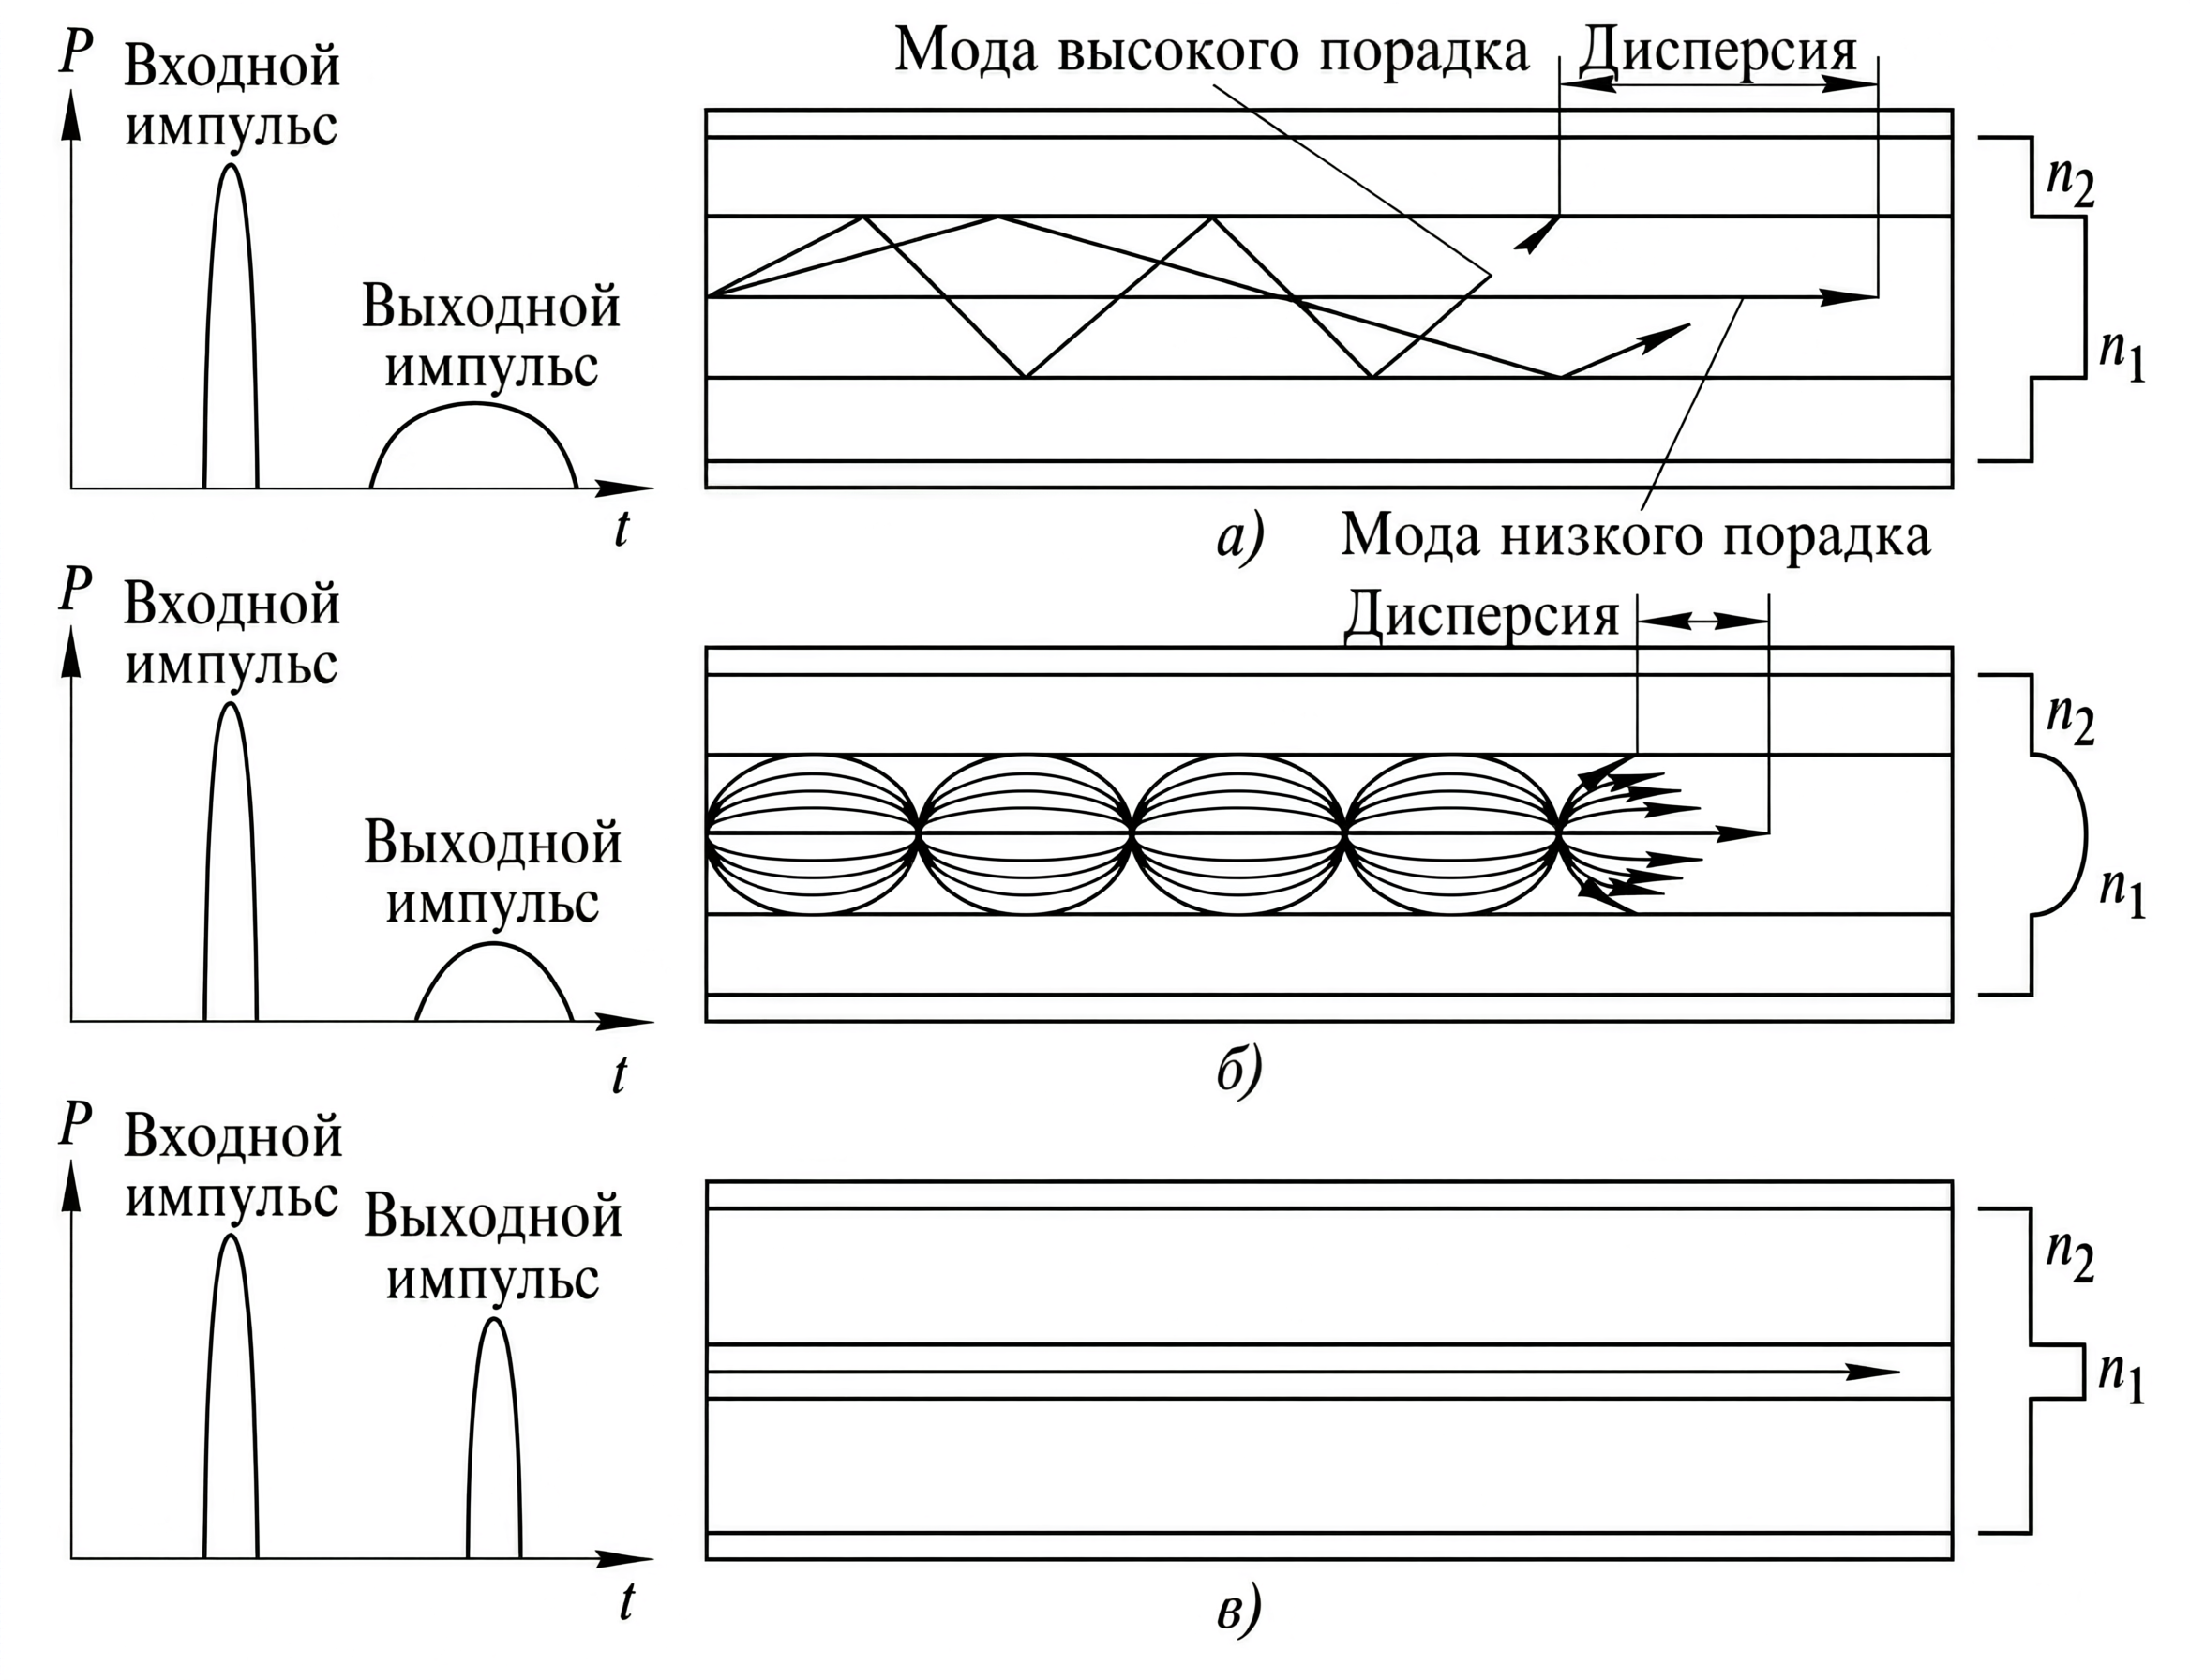
\includegraphics[width=0.8\textwidth]{rasprostranenie.png}
    \caption{Распространение излучения по ступенчатому и градиентному многомодовым, а также одномодовому оптическому волокну ~\cite{volokonno2012}}
    \label{fig:rasprostr}
\end{figure}

\subsubsubsection{Межмодовая дисперсия}

Межмодовая дисперсия преобладает в многомодовых ОВ и обусловлена различием групповых задержек большого числа направляемых мод. Для ОВ со ступенчатым профилем показателя преломления (ППП) фазовая скорость электромагнитной волны в сердцевине постоянна и равна:
\begin{equation}
    v = \frac{c}{n_1},
\end{equation}
где $c$ - скорость света в вакууме; $n_1$ - показатель преломления сердцевины.

Меридиональные лучи, входящие в торец ОВ под различными углами $\theta_n$ в пределах апертурного угла $\theta_A$, проходят различные зигзагообразные траектории. При одинаковой скорости распространения лучи достигают приемного конца в разное время, что приводит к уширению импульса. Согласно законам геометрической оптики, время распространения луча зависит от угла падения $\theta_n$ ~\cite{volokonno2012}:
\begin{equation}
    t = \frac{L \cdot n_1}{c \cdot \cos\theta_n},
\end{equation}
где $L$ - длина световода.

Минимальное время распространения соответствует осевому лучу ($\theta_n = 0$), а максимальное - лучу, распространяющемуся под критическим углом ($\theta_n = \theta_\text{кр}$) ~\cite{volokonno2012}:
\begin{equation}
    t_\text{мин} = \frac{L \cdot n_1}{c}, \quad t_\text{макс} = \frac{L \cdot n_1}{c \cdot \cos\theta_\text{кр}}.
\end{equation}
Межмодовая дисперсия $\tau_\text{мм}$ определяется как разность этих времен:
\begin{equation}
    \tau_\text{мм} = t_\text{макс} - t_\text{мин} = \frac{L \cdot n_1}{c} \left( \frac{1}{\cos\theta_\text{кр}} - 1 \right) \approx \frac{L \cdot n_1 \Delta}{c},
\end{equation}
где $\Delta = \frac{n_1 - n_2}{n_1}$ - относительная разность показателей преломления.

Из полученного выражения следует, что межмодовая дисперсия линейно возрастает с увеличением длины волокна. Однако это справедливо лишь для коротких участков, где отсутствует взаимодействие мод. В реальных условиях микроизгибы, неоднородности и кручение волокна вызывают постоянный обмен энергией между модами (перемешивание мод). В результате дисперсия становится пропорциональной $\sqrt{L}$. Этот эффект проявляется на расстояниях, превышающих \textit{длину установления модового равновесия} (эмпирически составляет 5-7~км для ступенчатых и 10-15~км для градиентных волокон~\cite{sklyarov2016}).

В градиентных многомодовых волокнах показатель преломления плавно убывает от оси к оболочке. Благодаря этому лучи, проходящие более длинные траектории на периферии, распространяются в среде с меньшим показателем преломления и, следовательно, с большей скоростью. Это компенсирует разность геометрических путей и существенно снижает дисперсию. Для параболического профиля ($u = 2$) уширение импульса составляет ~\cite{volokonno2012}:
\begin{equation}
    \tau_\text{мод} = \frac{L \cdot n_1 \Delta^2}{2c}.
\end{equation}

Минимальный разброс групповых задержек достигается при оптимальном значении параметра профиля~\cite{volokonno2012} $u_\text{опт} = 2(1 - \Delta)$, при котором дисперсия принимает минимальное значение (рисунок~\ref{fig:zavis})~\cite{volokonno2012}:
\begin{equation}
    \tau_\text{мод} = \frac{L \cdot n_1 \Delta^2}{8c}.
\end{equation}

\begin{figure}[h]
    \centering
    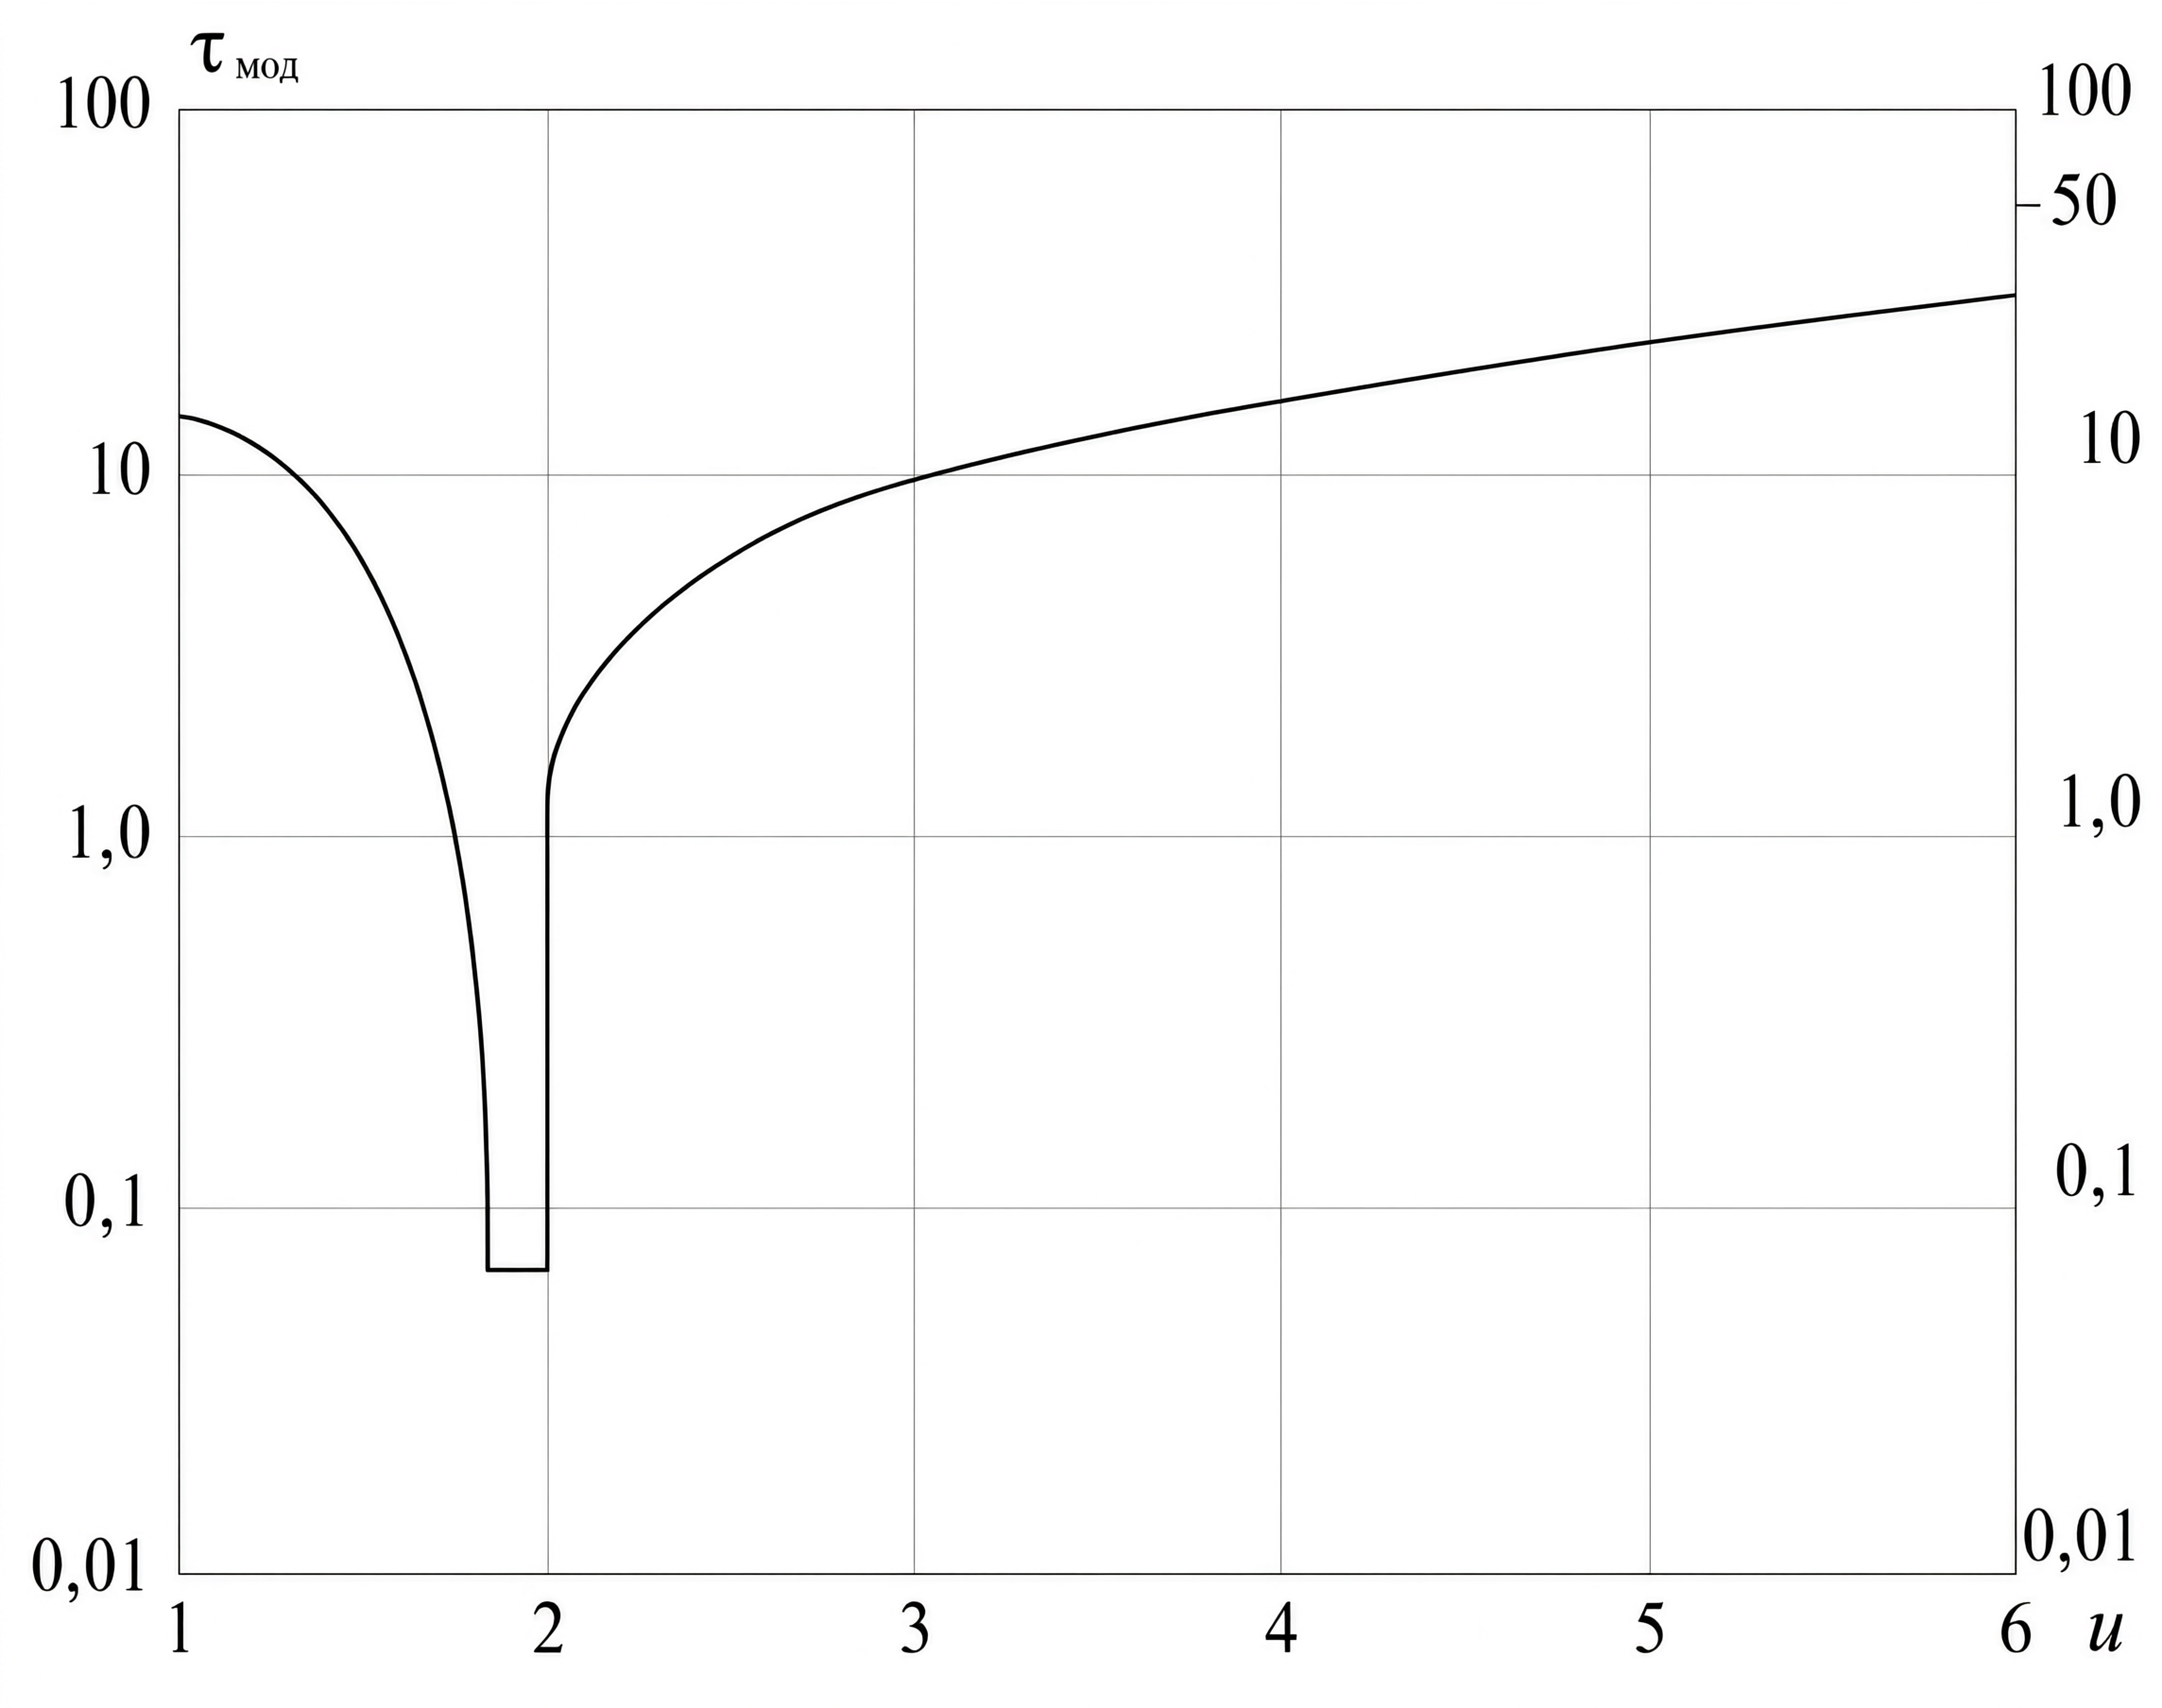
\includegraphics[width=0.8\textwidth]{zavisimost.png}
    \caption{Зависимость межмодовой дисперсии градиентного волокна от параметра профиля $u$ (без учета перемешивания мод)~\cite{volokonno2012}}
    \label{fig:zavis}
\end{figure}

Анализ показывает, что межмодовая дисперсия градиентного ОВ примерно в $\Delta/2$ раз меньше, чем у ступенчатого. Поскольку для стандартных волокон $\Delta \approx 1~\%$, выигрыш в полосе пропускания градиентных волокон достигает двух порядков.

Межмодовая дисперсия может быть минимизирована следующими методами:
\begin{enumerate}
    \item уменьшением диаметра сердцевины, что снижает число направляемых мод;
    \item оптимизацией профиля показателя преломления (использованием градиентных волокон) для выравнивания групповых задержек;
    \item переходом к одномодовому режиму передачи, при котором межмодовая дисперсия отсутствует.
\end{enumerate}

\subsubsubsection{Хроматическая дисперсия}

Хроматическая (частотная) дисперсия обусловлена зависимостью групповой скорости направляемой моды от длины волны излучения $\lambda$. Поскольку реальные источники излучения обладают конечной шириной спектра $\Delta\lambda$, различные спектральные компоненты сигнала распространяются с разными скоростями, что приводит к уширению импульса.

Хроматическая дисперсия складывается из материальной дисперсии материала сердцевины и волноводной (внутримодовой) дисперсии, обусловленной направляющими свойствами структуры ОВ.

Волноводная дисперсия $\tau_\text{вв}$ пропорциональна ширине спектра источника и длине линии~\cite{volokonno2012}:
\begin{equation}
    \tau_\text{вв} = \Delta\lambda \cdot L \cdot B(\lambda),
\end{equation}
где $B(\lambda)$ - удельная волноводная дисперсия. При отсутствии точных данных $B(\lambda)$ оценка $\tau_\text{вв}$ может быть выполнена по формуле~\cite{volokonno2012}:
\begin{equation}
    \tau_\text{вв} = \frac{\Delta\lambda}{\lambda} \cdot \frac{2 n_1^2 \Delta L}{c},
\end{equation}
где $\Delta\lambda$ --- ширина спектра источника в рабочем режиме.

\subsubsubsection{Материальная дисперсия}

Материальная дисперсия обусловлена зависимостью показателя преломления материала сердцевины от длины волны $n(\lambda)$. В диспергирующей среде фазовая и групповая скорости зависят от частоты, поэтому различные спектральные компоненты одного и того же источника проходят волокно за разное время.

Характер материальной дисперсии определяется рабочей длиной волны. В области 850~нм более длинные волны распространяются быстрее коротких (нормальная дисперсия). В области 1550~нм ситуация обратная: более короткие волны опережают длинные (аномальная дисперсия). При некотором значении $\lambda_0 \approx 1{,}27 \dots 1{,}30$~мкм материальная дисперсия обращается в ноль~\cite{volokonno2012}. Эта длина волны называется \textit{длиной волны нулевой дисперсии}.

Материальная дисперсия $\tau_\text{мат}$ рассчитывается по выражению~\cite{volokonno2012}:
\begin{equation}
    \tau_\text{мат} = \Delta\lambda \cdot L \cdot M(\lambda),
\end{equation}
где $M(\lambda)$ - коэффициент материальной дисперсии, зависящий от состава легирующих примесей и определяемый экспериментально или из справочных данных.

\subsubsubsection{Поляризационная модовая дисперсия}

Поляризационная модовая дисперсия (ПМД) $\tau_\text{пмд}$ возникает вследствие различия скоростей распространения двух взаимно ортогональных поляризаций основной моды $HE_{11}$ в одномодовом волокне. Для оценки ПМД используется выражение~\cite{volokonno2012}:
\begin{equation}
    \tau_\text{пмд} = K_\text{пмд} \sqrt{L},
\end{equation}
где $K_\text{пмд}$ - коэффициент удельной поляризационной модовой дисперсии (пс/$\sqrt{\text{км}}$).

В идеальном волокне с идеальной круглой симметрией обе поляризации вырождены. Однако в реальных ОВ наличие эллиптичности сердцевины, внутренних напряжений и внешних изгибов приводит к возникновению собственного двойного лучепреломления. ПМД становится критичной при передаче высокоскоростных сигналов (10~Гбит/с и выше~\cite{sklyarov2016}) на большие расстояния.

Результирующая полная дисперсия одномодового волокна определяется с учетом хроматической и поляризационной составляющих~\cite{volokonno2012}:
\begin{equation}
    \tau = \sqrt{(\tau_\text{вв} + \tau_\text{мат})^2 + \tau_\text{пмд}^2}.
\end{equation}
В стандартных условиях эксплуатации $K_\text{пмд}$ достаточно мало, и вкладом ПМД в суммарное уширение часто можно пренебречь.

В реальном одномодовом волокне вследствие анизотропии
две ортогональные поляризации могут иметь разные постоянные
распространения. На рисунке~\ref{fig:PMD} показано,
как разность их групповых задержек влияет на форму импульса.
\begin{figure}[h]
    \centering
    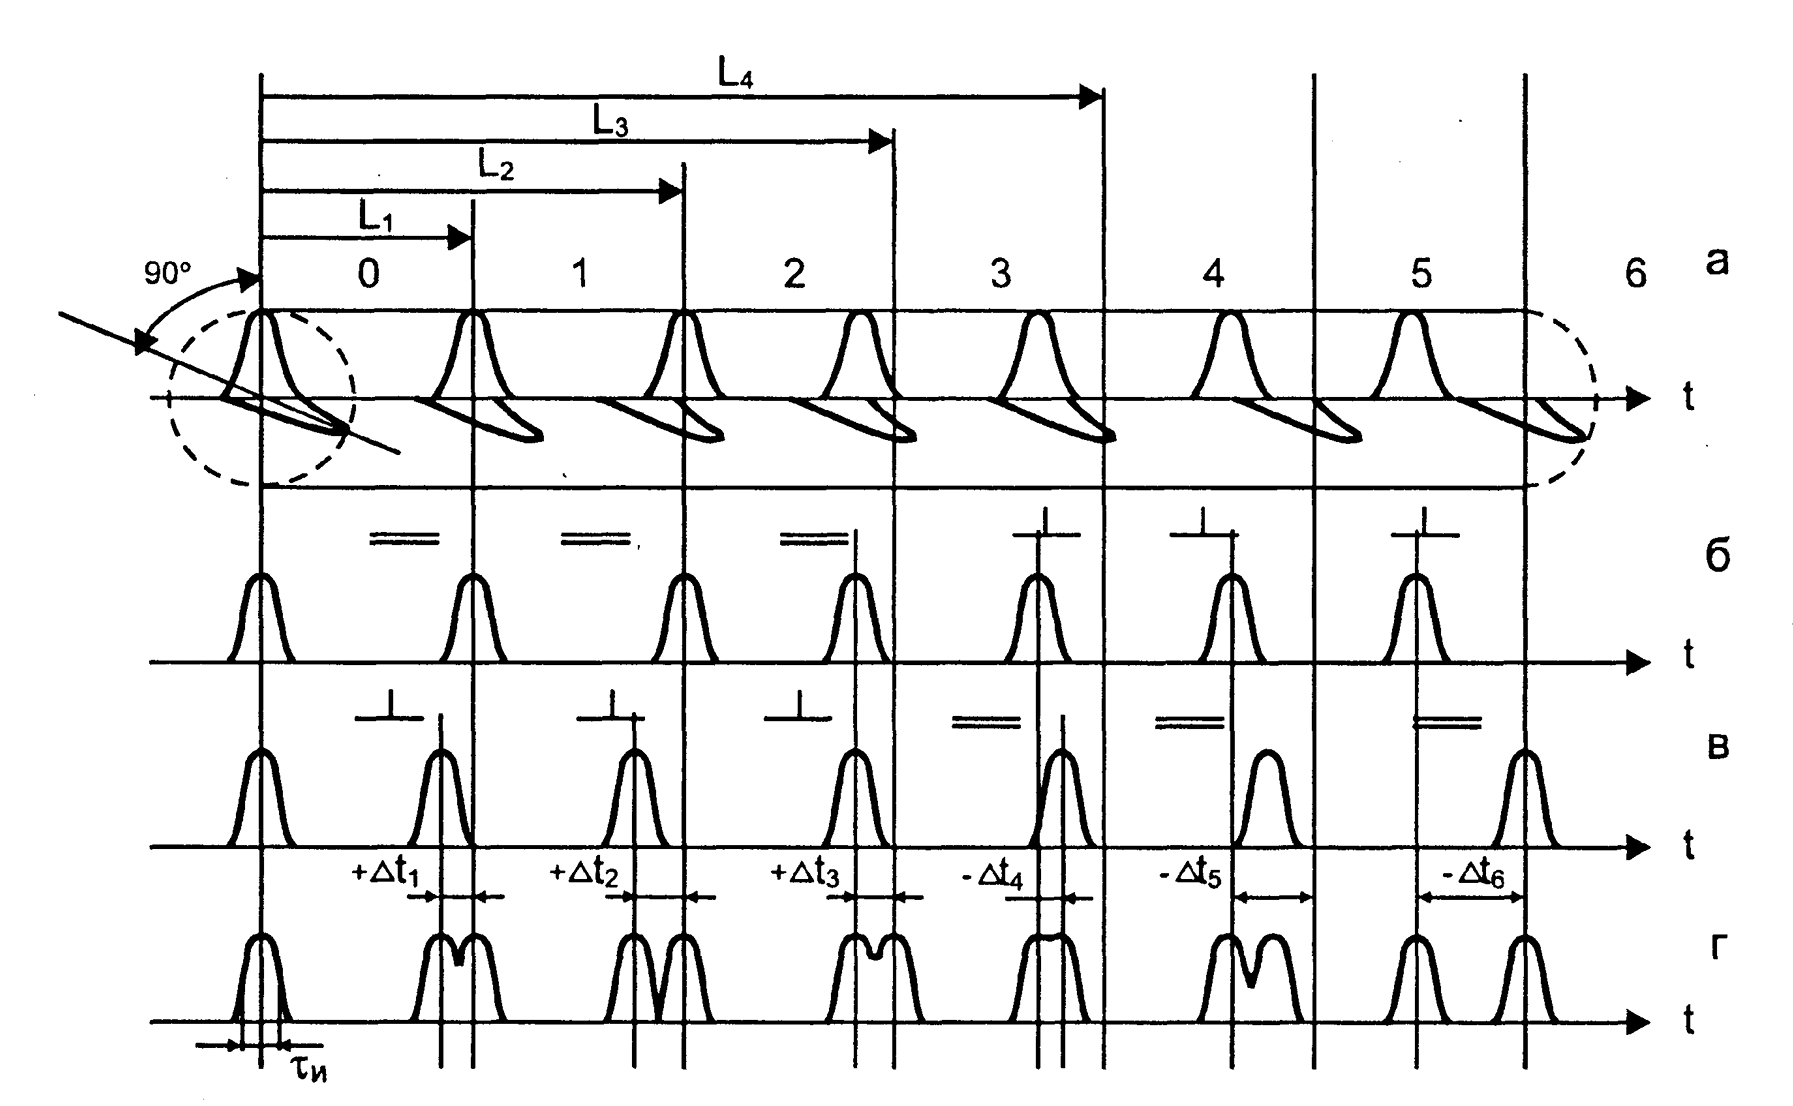
\includegraphics[width=0.8\textwidth]{PMD.png}
    \caption{Механизм расширения импульса за счет ПМД~\cite{sklyarov2016}}
    \label{fig:PMD}
\end{figure}

Разность задержек поляризационных составляющих может привести
к раздвоению импульса, если она превышает его начальную
длительность. В длинном волокне с меняющейся анизотропией
поляризации перемешиваются. Статистическое накопление задержек
на слабо коррелированных участках объясняет зависимость
характерной дифференциальной задержки от \(\sqrt L\)~\cite{sklyarov2016}.

В многомодовых ОВ волноводная дисперсия мала, поэтому ею пренебрегают. Для ступенчатых многомодовых волокон доминирует межмодовая дисперсия, а для градиентных - материальная (поскольку межмодовая компенсирована профилем). Полная дисперсия многомодового волокна~\cite{volokonno2012}:
\begin{equation}
    \tau = \sqrt{\tau_\text{мод}^2 + \tau_\text{мат}^2}.
\end{equation}

Сравнение дисперсионных характеристик показывает, что наименьшее уширение импульсов обеспечивают одномодовые ОВ, в то время как наиболее сильная дисперсия наблюдается в многомодовых волокнах со ступенчатым профилем показателя преломления.

\clearpage

\section{ПРАКТИЧЕСКАЯ ЧАСТЬ}
\subsection{Установка и записи}

Импульсы лазера SWLD-1554.94-FC/PC-05-PM с длиной волны
\(1554{,}94\) нм делились первым планарным разветвителем между
коротким плечом и плечом с катушкой. Второй разветвитель подавал
обе копии на аналоговый InGaAs-фотоприёмник FPD310-FC-NIR
с усилителем. Осциллограммы записаны на LeCroy WaveRunner 44Xi.
Схема установки приведена на рисунке~\ref{fig:setup}.

\begin{figure}[htbp]
  \centering
  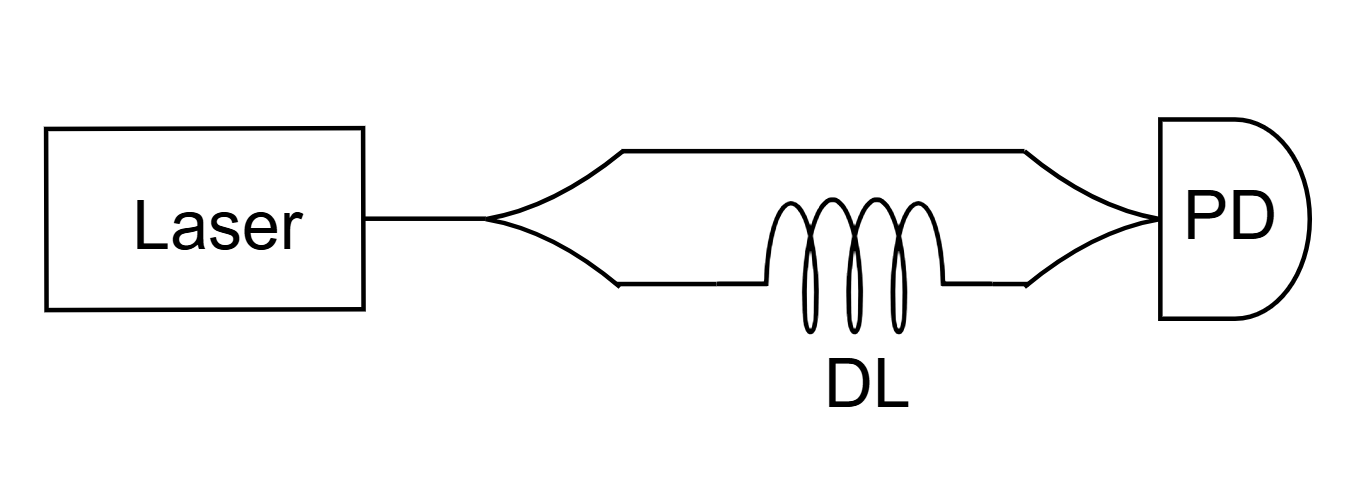
\includegraphics[width=0.68\linewidth]{Setup.png}
  \caption{Схема установки. Laser обозначает лазер, DL --- линию
    задержки, PD --- фотоприёмник}
  \label{fig:setup}
\end{figure}

Файл \texttt{C2300000.txt} содержит оба импульса на одной временной
шкале с шагом \(\OverviewStep\) нс. Для интегрирования использованы
отдельные записи с шагом \(\FineStep\) нс. По порядку регистрации
\texttt{C2300001.txt} отнесён к короткому плечу, а
\texttt{C2300002.txt} --- к плечу с катушкой. Временной ноль
у каждой подробной записи свой. Все результаты ниже рассчитаны
по этой серии.

\subsection{Задержка и длина линии}

В общей записи найдены максимальные отсчёты до и после
\(t=1\) мкс. Их времена \(t_1=\PeakEarly\) и \(t_2=\PeakLate\) мкс
отмечены на рисунке~\ref{fig:delay}. При отнесении обоих пиков
к одному оптическому запуску разность \(t_2-t_1\) даёт групповую
задержку длинного плеча относительно короткого. Для волокна
групповая скорость \(v_g=c/n_g\), где \(n_g\) --- групповой
показатель преломления, \(c\) --- скорость света в вакууме~\cite{agrawal}.

\begin{figure}[htbp]
  \centering
  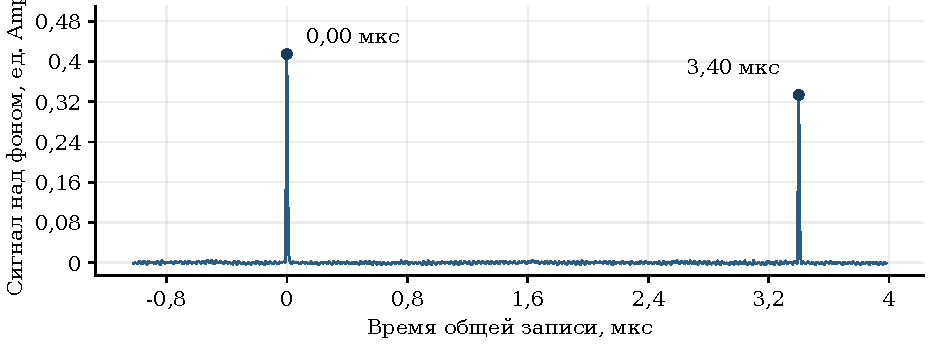
\includegraphics[width=\linewidth]{delay.pdf}
  \caption{Общая осциллограмма \texttt{C2300000.txt} после вычитания
    среднего уровня при \(t<-0{,}10\) мкс. Маркеры показывают
    максимальные отсчёты двух импульсов}
  \label{fig:delay}
\end{figure}

\begin{samepage}
Если разность длин плеч определяется катушкой, оценка её длины
при принятом \(n_g=\GroupIndex\) составляет
\begin{equation}
  \Delta t=t_2-t_1=\PeakDelay~\text{мкс},\qquad
  L\simeq\frac{c\,\Delta t}{n_g}\simeq\LengthMeters~\text{м}.
  \label{eq:length}
\end{equation}
\end{samepage}
При условии, что вершина каждого импульса лежит между соседями
отсчёта максимума, сдвиг \(\Delta t\) из-за сетки может составить
до \(2\cdot\OverviewStep=20\) нс по модулю. Это даёт диапазон
\(\DelayLower\)--\(\DelayUpper\) мкс для задержки и
\(\LengthLower\)--\(\LengthUpper\) м для длины при том же \(n_g\).
Для сравнения, при \(n_g=\ReferenceIndex\), паспортном значении
SMF-28 Ultra при \(1550\) нм, формула~\eqref{eq:length}
даёт \(\ReferenceLength\) м. Это иллюстрирует чувствительность
к выбору показателя преломления~\cite{corning}.

\subsection{Ослабление по площадям импульсов}

Обозначим \(u_0(t)\) и \(u_L(t)\) сигналы короткого плеча и плеча
с катушкой. Для каждого сигнала фоновый уровень \(b_j\) взят как
среднее всех отсчётов до \(t=\BackgroundLimit\) нс включительно
по шкале своего файла. Эта граница лежит до начала подъёма обоих
импульсов. Из каждого отсчёта вычтен соответствующий фон,
\(p_j(t)=u_j(t)-b_j\). В таблице~\ref{tab:areas} указаны
число фоновых отсчётов \(N_b\) и найденные уровни \(b_j\).

Обозначим \(t_{f,j}\) время пересечения передним фронтом половины
собственного максимума \(p_j\). Пересечение найдено линейной
интерполяцией между соседними отсчётами. Площади обоих импульсов
вычислены в одинаковом окне \([\WindowStart;\WindowEnd]\) нс
относительно \(t_{f,j}\) по правилу трапеций с интерполяцией
в точках границы. Нижняя граница лежит перед фронтом, верхняя
захватывает спад и общую наблюдаемую часть хвоста. Амплитудный
масштаб сохранён при совмещении фронтов, как на рисунке~\ref{fig:pulses}.

\begin{figure}[htbp]
  \centering
  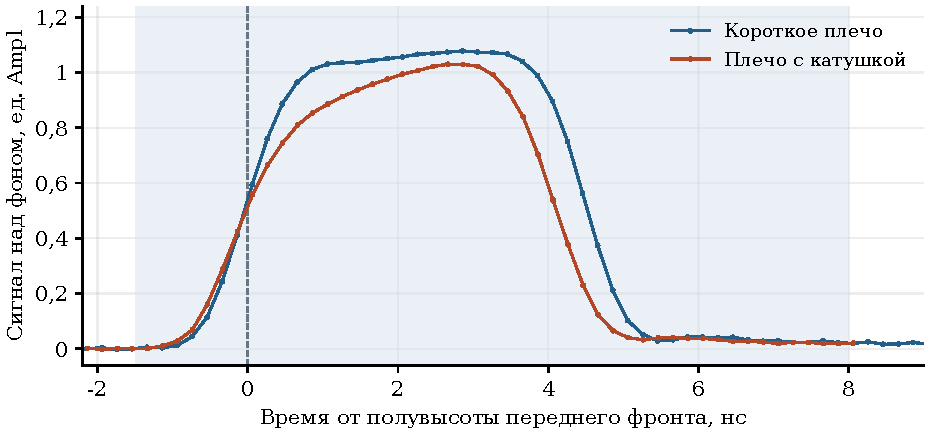
\includegraphics[width=\linewidth]{pulses.pdf}
  \caption{Импульсы из \texttt{C2300001.txt} и \texttt{C2300002.txt}
    после вычитания фона. Окно интегрирования выделено заливкой,
    штриховая линия отмечает полувысоту переднего фронта по времени}
  \label{fig:pulses}
\end{figure}

\begin{equation}
  S_j=\int_{\WindowStart~\text{нс}}^{\WindowEnd~\text{нс}}
        p_j(t_{f,j}+\tau)\,\dd\tau,\qquad
  \eta=\frac{S_L}{S_0},\qquad
  A=10\lg\frac{S_0}{S_L}.
  \label{eq:attenuation}
\end{equation}

\begin{table}[htbp]
  \caption{Фоновые уровни и площади импульсов}
  \label{tab:areas}
  \centering
  \small
  \begin{tabular}{lrrrr}
    \toprule
    Плечо & \(N_b\) & \(b_j\), ед. Ampl & \(t_{f,j}\), нс & \(S_j\), ед. Ampl \(\cdot\) нс\\
    \midrule
    \PulseRows
    \bottomrule
  \end{tabular}
\end{table}

В линейном режиме фотоприёмника сигнал создаёт падающая оптическая
мощность \(P_j(t)\). Входная оптическая энергия импульса
равна \(\int P_j(t)\dd t\), поэтому для отношения энергий
используется \(10\lg\), без возведения сигнала в квадрат.
На выходе FPD310 установлена развязка по постоянному току~\cite{menlo}.

При линейной регистрации \(p_j\) описывается свёрткой \(G(h*P_j)\)
с электрическим откликом \(h\) и усилением \(G\). Если оптические
импульсы отличаются только множителем и сдвигом и зарегистрированы
при одном \(G\) и \(h\), такой же множитель получится для
площадей в одинаково совмещённых окнах. Здесь формы отличаются,
поэтому \(\eta\) служит оценкой относительной передачи по площадям
зарегистрированных импульсов.

Получено \(\eta=\AreaRatio\), что соответствует
\(A\simeq\PathLoss\) дБ. Удельная оценка
\begin{equation}
  \alpha_{\text{эфф}}=\frac{A}{L_{\text{км}}}
    \simeq \EffectiveLoss~\text{дБ/км}
    \qquad (L_{\text{км}}\simeq\LengthKm).
\end{equation}
Сравнение ветвей предполагает одинаковые настройки регистрации
и одинаковую энергию запуска в двух отдельных записях.
Если обозначить через \(K_0,K_L\) оптическую передачу портов
разветвителей и соединений соответствующих плеч вне катушки,
энергия на приёмнике в длинном плече по отношению к короткому
равна \((K_L/K_0)10^{-A_{\text{кат}}/10}\), где \(A_{\text{кат}}\)
включает потери сборки катушки. Таким образом, при сопоставимом
электрическом отклике \(A\simeq A_{\text{кат}}+10\lg(K_0/K_L)\).
При \(K_0=K_L\) эта оценка соответствует вносимому ослаблению
катушки. Передача портов в данной серии отдельно не измерялась,
поэтому \(\alpha_{\text{эфф}}\) характеризует сравнение двух плеч.

\subsection{Чувствительность результата к обработке}

Таблица~\ref{tab:window} показывает изменение \(A\) при выборе
конца окна, границы фонового участка и способа оценки уровня
фона. В каждом варианте нижняя граница окна равна
\(\WindowStart\) нс и совмещение фронтов повторено после вычитания
фона. Каждое окно заканчивается после пересечения полувысоты
на спаде обоих импульсов.
Ослабление меняется от \(0{,}68\) до \(0{,}70\) дБ. Этот
разброс характеризует чувствительность к обработке.
Неопределённость передачи портов и возможного
различия настроек регистрации по этим записям оценить нельзя.

\begin{table}[htbp]
  \caption{Зависимость ослабления от выбора окна и фона}
  \label{tab:window}
  \centering
  \small
  \begin{tabular}{r l r r}
    \toprule
    Конец окна, нс & Оценка фона & Граница фона, нс & \(A\), дБ\\
    \midrule
    \SensitivityRows
    \bottomrule
  \end{tabular}
\end{table}

\FloatBarrier
\section*{ЗАКЛЮЧЕНИЕ}
\phantomsection
\addcontentsline{toc}{section}{ЗАКЛЮЧЕНИЕ}

По двум пикам на общей осциллограмме найдена задержка
\(\PeakDelay\) мкс. Она соответствует длине линии около
\(\LengthMeters\) м при \(n_g=\GroupIndex\).

После вычитания фона и интегрирования подробных осциллограмм
в общем временном окне площадь импульса в плече с катушкой
составила \(\AreaRatio\) от площади импульса короткого плеча.
Это даёт ослабление около \(\PathLoss\) дБ и эффективное
удельное значение \(\EffectiveLoss\) дБ/км для сравнения плеч.
Чтобы выделить вклад волокна, требуется отдельно определить
передачу портов и соединений и проверить отклик фотоприёмника.

\clearpage
\phantomsection
\addcontentsline{toc}{section}{СПИСОК ИСПОЛЬЗОВАННЫХ ИСТОЧНИКОВ}
\begin{thebibliography}{9}
\raggedright
\bibitem{Slepov}
Слепов Н.\,Н. Современные технологии цифровых оптоволоконных сетей
связи. М., Радио и связь, 2000. С.~9--24, 384--394, 412--416.

\bibitem{Burdin}
Бурдин А.\,В. Многомодовые оптические волокна в современной кабельной
инфраструктуре российских инфокоммуникационных сетей.
Электросвязь, 2010, №~4. С.~24--27.

\bibitem{volokonno2012}
Родина О.\,В. Волоконно-оптические линии связи.
М., Горячая линия--Телеком, 2012. С.~7--63.

\bibitem{velichansky2007}
Величанский В.\,Л., Егоров В.\,К. Лабораторный практикум
«Волоконно-оптическая линия связи». М., МИФИ, 2008. С.~3--51.

\bibitem{sklyarov2016}
Скляров О.\,К. Волоконно-оптические сети и системы связи.
3-е изд., стер. СПб., Лань, 2016. С.~100--214.

\bibitem{agrawal}
Агравал Г. Нелинейная волоконная оптика. Пер. с англ.
М., Мир, 1996. \S\,1.2.2--1.2.3.

\bibitem{menlo}
Menlo Systems. FPD310: High Sensitivity Fast PIN Photodetector.
Техническое описание. \url{https://menlosystems.com/downloads/fpd310-datasheet-en/}

\bibitem{corning}
Corning. SMF-28 Ultra Optical Fiber: Product Information PI-1424-AEN.
Техническое описание. \url{https://corning.com/opticalfiber}
\end{thebibliography}
\end{document}
